%%%%%%%%%%%%%%%%%%%%%%%%%%%%%%%%%%%%%%%%%
% Masters/Doctoral Thesis 
% LaTeX Template
% Version 1.43 (17/5/14)
%
% This template has been downloaded from:
% http://www.LaTeXTemplates.com
%
% Original authors:
% Steven Gunn 
% http://users.ecs.soton.ac.uk/srg/softwaretools/document/templates/
% and
% Sunil Patel
% http://www.sunilpatel.co.uk/thesis-template/
%
% License:
% CC BY-NC-SA 3.0 (http://creativecommons.org/licenses/by-nc-sa/3.0/)
%
% Note:
% Make sure to edit document variables in the Thesis.cls file
%
%%%%%%%%%%%%%%%%%%%%%%%%%%%%%%%%%%%%%%%%%

%----------------------------------------------------------------------------------------
%	PACKAGES AND OTHER DOCUMENT CONFIGURATIONS
%----------------------------------------------------------------------------------------

\documentclass[11pt, oneside]{Thesis} % The default font size and one-sided printing (no margin offsets)

\graphicspath{{Pictures/}} % Specifies the directory where pictures are stored

\usepackage[square, numbers, comma, sort&compress]{natbib} % Use the natbib reference package - read up on this to edit the reference style; if you want text (e.g. Smith et al., 2012) for the in-text references (instead of numbers), remove 'numbers' 
\usepackage{listings}
\hypersetup{urlcolor=blue, colorlinks=true} % Colors hyperlinks in blue - change to black if annoying
\title{\ttitle} % Defines the thesis title - don't touch this

\begin{document}

\frontmatter % Use roman page numbering style (i, ii, iii, iv...) for the pre-content pages

\setstretch{1.3} % Line spacing of 1.3

% Define the page headers using the FancyHdr package and set up for one-sided printing
\fancyhead{} % Clears all page headers and footers
\rhead{\thepage} % Sets the right side header to show the page number
\lhead{} % Clears the left side page header

\pagestyle{fancy} % Finally, use the "fancy" page style to implement the FancyHdr headers

\newcommand{\HRule}{\rule{\linewidth}{0.5mm}} % New command to make the lines in the title page

% PDF meta-data
\hypersetup{pdftitle={\ttitle}}
\hypersetup{pdfsubject=\subjectname}
\hypersetup{pdfauthor=\authornames}
\hypersetup{pdfkeywords=\keywordnames}
% ADDED BY MAGNUS 

%----------------------------------------------------------------------------------------
%	TITLE PAGE
%----------------------------------------------------------------------------------------

\begin{titlepage}
\begin{center}

\textsc{\LARGE \univname}\\[1.5cm] % University name
\textsc{\Large Project TMA4500}\\[0.5cm] % Thesis type

\HRule \\[0.4cm] % Horizontal line
{\huge \bfseries \ttitle}\\[0.4cm] % Thesis title
\HRule \\[1.5cm] % Horizontal line
 
\begin{minipage}{0.4\textwidth}
\begin{flushleft} \large
\emph{Author:}\\
\href{http://www.johnsmith.com}{\authornames} % Author name - remove the \href bracket to remove the link
\end{flushleft}
\end{minipage}
\begin{minipage}{0.4\textwidth}
\begin{flushright} \large
\emph{Supervisor:} \\
\href{http://www.jamessmith.com}{\supname} % Supervisor name - remove the \href bracket to remove the link  
\end{flushright}
\end{minipage}\\[3cm]
 
%\large \textit{A thesis submitted in fulfilment of the requirements\\ for the degree of \degreename}\\[0.3cm] % University requirement text
%\textit{in the}\\[0.4cm]
\groupname\\\deptname\\[2cm] % Research group name and department name
 
{\large \today}\\[4cm] % Date
%\includegraphics{Logo} % University/department logo - uncomment to place it
 
\vfill
\end{center}

\end{titlepage}
%%fakesection - Declaration of Authorship
%----------------------------------------------------------------------------------------
%	DECLARATION PAGE
%	Your institution may give you a different text to place here
%----------------------------------------------------------------------------------------
%\Declaration{

%\addtocontents{toc}{\vspace{1em}} % Add a gap in the Contents, for aesthetics

%I, \authornames, declare that this thesis titled, '\ttitle' and the work presented in it are my own. I confirm that:

%\begin{itemize} 
%\item[\tiny{$\blacksquare$}] This work was done wholly or mainly while in candidature for a research degree at this University.
%\item[\tiny{$\blacksquare$}] Where any part of this thesis has previously been submitted for a degree or any other qualification at this University or any other institution, this has been clearly stated.
%\item[\tiny{$\blacksquare$}] Where I have consulted the published work of others, this is always clearly attributed.
%\item[\tiny{$\blacksquare$}] Where I have quoted from the work of others, the source is always given. With the exception of such quotations, this thesis is entirely my own work.
%\item[\tiny{$\blacksquare$}] I have acknowledged all main sources of help.
%\item[\tiny{$\blacksquare$}] Where the thesis is based on work done by myself jointly with others, I have made clear exactly what was done by others and what I have contributed myself.\\
%\end{itemize}
 
%Signed:\\
%\rule[1em]{25em}{0.5pt} % This prints a line for the signature
 
%Date:\\
%\rule[1em]{25em}{0.5pt} % This prints a line to write the date
%}

%\clearpage % Start a new page
%%fakesection - Quotation page
%----------------------------------------------------------------------------------------
%	QUOTATION PAGE
%----------------------------------------------------------------------------------------

%\pagestyle{empty} % No headers or footers for the following pages

%\null\vfill % Add some space to move the quote down the page a bit

%\textit{``Thanks to my solid academic training, today I can write hundreds of words on virtually any topic without possessing a shred of information, which is how I got a good job in journalism."}

%\begin{flushright}
%Dave Barry
%\end{flushright}

%\vfill\vfill\vfill\vfill\vfill\vfill\null % Add some space at the bottom to position the quote just right

%\clearpage % Start a new page

%----------------------------------------------------------------------------------------
%	ABSTRACT PAGE
%----------------------------------------------------------------------------------------
%%fakesection - Abstract
\addtotoc{Abstract} % Add the "Abstract" page entry to the Contents

\abstract{\addtocontents{toc}{\vspace{1em}} % Add a gap in the Contents, for aesthetics
In this project some basic properties of the least squares method is analysed. Both finite element and spectral methods are discussed, and the implementation is mainly performed using spectral basis functions. The problems analysed in this project are diffusion convection reaction PDEs, both linear and non-linear. The results are compared to standard Galerkin method where both error and condition number is considered. The least squares method is also applied to Galerkin methods to gain stability with great results.  
}

\clearpage % Start a new page

%%fakesection - Acknowledgements 
%----------------------------------------------------------------------------------------
%	ACKNOWLEDGEMENTS
%----------------------------------------------------------------------------------------

%\setstretch{1.3} % Reset the line-spacing to 1.3 for body text (if it has changed)

%\acknowledgements{\addtocontents{toc}{\vspace{1em}} % Add a gap in the Contents, for aesthetics

%The acknowledgements and the people to thank go here, don't forget to include your project advisor\ldots
%}
%\clearpage % Start a new page

%%fakesection - List of contents/figs/tables
%----------------------------------------------------------------------------------------
%	LIST OF CONTENTS/FIGURES/TABLES PAGES
%----------------------------------------------------------------------------------------

\pagestyle{fancy} % The page style headers have been "empty" all this time, now use the "fancy" headers as defined before to bring them back

\lhead{\emph{Contents}} % Set the left side page header to "Contents"
\tableofcontents % Write out the Table of Contents

%\lhead{\emph{List of Figures}} % Set the left side page header to "List of Figures"
%\listoffigures % Write out the List of Figures

%\lhead{\emph{List of Tables}} % Set the left side page header to "List of Tables"
%\listoftables % Write out the List of Tables

%%fakesection - Abbreviations
%----------------------------------------------------------------------------------------
%	ABBREVIATIONS
%----------------------------------------------------------------------------------------

%\clearpage % Start a new page

%\setstretch{1.5} % Set the line spacing to 1.5, this makes the following tables easier to read

%\lhead{\emph{Abbreviations}} % Set the left side page header to "Abbreviations"
%\listofsymbols{ll} % Include a list of Abbreviations (a table of two columns)
%{
%\textbf{LAH} & \textbf{L}ist \textbf{A}bbreviations \textbf{H}ere \\
%%\textbf{Acronym} & \textbf{W}hat (it) \textbf{S}tands \textbf{F}or \\
%}

%%fakesection - Constants/Definitions 
%----------------------------------------------------------------------------------------
%	PHYSICAL CONSTANTS/OTHER DEFINITIONS
%----------------------------------------------------------------------------------------

%\clearpage % Start a new page

%\lhead{\emph{Physical Constants}} % Set the left side page header to "Physical Constants"

%\listofconstants{lrcl} % Include a list of Physical Constants (a four column table)
%{
%Speed of Light & $c$ & $=$ & $2.997\ 924\ 58\times10^{8}\ \mbox{ms}^{-\mbox{s}}$ (exact)\\
%% Constant Name & Symbol & = & Constant Value (with units) \\
%}

%%fakesection - Symbols 
%----------------------------------------------------------------------------------------
%	SYMBOLS
%----------------------------------------------------------------------------------------

%\clearpage % Start a new page

%\lhead{\emph{Symbols}} % Set the left side page header to "Symbols"

%\listofnomenclature{lll} % Include a list of Symbols (a three column table)
%{
%$a$ & distance & m \\
%$P$ & power & W (Js$^{-1}$) \\
%% Symbol & Name & Unit \\

%& & \\ % Gap to separate the Roman symbols from the Greek

%$\omega$ & angular frequency & rads$^{-1}$ \\
%% Symbol & Name & Unit \\
%}

%%fakesection - Dedication
%----------------------------------------------------------------------------------------
%	DEDICATION
%----------------------------------------------------------------------------------------

%\setstretch{1.3} % Return the line spacing back to 1.3

%\pagestyle{empty} % Page style needs to be empty for this page

%\dedicatory{For/Dedicated to/To my\ldots} % Dedication text

%\addtocontents{toc}{\vspace{2em}} % Add a gap in the Contents, for aesthetics

%----------------------------------------------------------------------------------------
%	THESIS CONTENT - CHAPTERS
%----------------------------------------------------------------------------------------

%%fakesection - Notation 
%----------------------------------------------------------------------------------------
%	NOTATION
%----------------------------------------------------------------------------------------

\clearpage % Start a new page

\setstretch{1.5} % Set the line spacing to 1.5, this makes the following tables easier to read

\lhead{\emph{Notation}} % Set the left side page header to "Abbreviations"
\listofsymbols{ll} % Include a list of Abbreviations (a table of two columns)
{
\textbf{CONVENTION} & we let subscript $h$ denote the discretized variables \\
%$u$ & Solution of the partial differential equation\\
%$\mathbf{w} = [w_1 \; w_2 ] $ & Negative gradient of $u$ \\
%$\mathbf{u} = [ \mathbf{w} \; u ]^T$ & Solution to the first order transformation \\ 
%$ R_g $ & Lifting function \\
%$\tilde{\mathbf{u}} = \mathbf{u}-R_g $ & Solution to the first order transformation minus the lifting function \\ 
%$\mathbf{b}$ & Two dimensional vector field \\
%$f$ & loading function\\
%$\mathbf{f} = (0,0,f)$ & loading function for the first order transformation\\
%$\mathcal{L} , \mathcal{B} $ & Linear operators \\
%$(\cdot,\cdot)$ & Inner product, when not specified read as $(\cdot,\cdot)_{L_2}$  \\
%$a(\cdot,\cdot)$ & Bilinear form obtained from standard Galerkin approach \\
%$Q(\cdot,\cdot)$ & Bilinear form obtained from the least squares approach \\
%$\mathring{a}(\cdot,\cdot)$ & Bilinear form obtained from the combined GLS-method\\
%$F(\cdot)$ & Linear form obtained from the least squares approach \\
%$\tilde{F}(\cdot)$ & Linear form obtained from the least squares approach including BC's \\
%$\mathring{F}(\cdot)$ & Linear form obtained from the combined GLS-method \\
%\textbf{Linear Algebra} \\
%$A$ & The stiffness matrix \\
%$G$ & The gradient matrix \\
%$R$ & The reaction matrix \\
%$F$ & The vector obtained from the linear functional $F(\cdot)$ \\ 
%$W$ 	& The diagonal matrix with the GLL-weights \\ 
%$L$ 	& The matrix with the derivative of the lagrange functions in each node \\ 
%$\Phi$ & $W\otimes WL$\\ 
%$\Psi$ & $WL\otimes W$\\ 

%\textbf{LAH} & \textbf{L}ist \textbf{A}bbreviations \textbf{H}ere \\
%\textbf{Acronym} & \textbf{W}hat (it) \textbf{S}tands \textbf{F}or \\
}

\mainmatter % Begin numeric (1,2,3...) page numbering

\pagestyle{fancy} % Return the page headers back to the "fancy" style

% Include the chapters of the thesis as separate files from the Chapters folder
% Uncomment the lines as you write the chapters

%% Chapter 1

\chapter{Chapter Title Here} % Main chapter title

\label{Chapter1} % For referencing the chapter elsewhere, use \ref{Chapter1} 

\lhead{Chapter 1. \emph{Chapter Title Here}} % This is for the header on each page - perhaps a shortened title

%----------------------------------------------------------------------------------------

\section{Welcome and Thank You}
Welcome to this \LaTeX{} Thesis Template, a beautiful and easy to use template for writing a thesis using the \LaTeX{} typesetting system.

If you are writing a thesis (or will be in the future) and its subject is technical or mathematical (though it doesn't have to be), then creating it in \LaTeX{} is highly recommended as a way to make sure you can just get down to the essential writing without having to worry over formatting or wasting time arguing with your word processor.

\LaTeX{} is easily able to professionally typeset documents that run to hundreds or thousands of pages long. With simple mark-up commands, it automatically sets out the table of contents, margins, page headers and footers and keeps the formatting consistent and beautiful. One of its main strengths is the way it can easily typeset mathematics, even \emph{heavy} mathematics. Even if those equations are the most horribly twisted and most difficult mathematical problems that can only be solved on a super-computer, you can at least count on \LaTeX{} to make them look stunning.

%----------------------------------------------------------------------------------------

\section{Learning \LaTeX{}}

\LaTeX{} is not a WYSIWYG (What You See is What You Get) program, unlike word processors such as Microsoft Word or Apple's Pages. Instead, a document written for \LaTeX{} is actually a simple, plain text file that contains \emph{no formatting}. You tell \LaTeX{} how you want the formatting in the finished document by writing in simple commands amongst the text, for example, if I want to use \textit{italic text for emphasis}, I write the `$\backslash$\texttt{textit}\{\}' command and put the text I want in italics in between the curly braces. This means that \LaTeX{} is a ``mark-up'' language, very much like HTML.

\subsection{A (not so short) Introduction to \LaTeX{}}

If you are new to \LaTeX{}, there is a very good eBook -- freely available online as a PDF file -- called, ``The Not So Short Introduction to \LaTeX{}''. The book's title is typically shortened to just ``lshort''. You can download the latest version (as it is occasionally updated) from here:\\
\href{http://www.ctan.org/tex-archive/info/lshort/english/lshort.pdf}{\texttt{http://www.ctan.org/tex-archive/info/lshort/english/lshort.pdf}}

It is also available in several other languages. Find yours from the list on this page:\\
\href{http://www.ctan.org/tex-archive/info/lshort/}{\texttt{http://www.ctan.org/tex-archive/info/lshort/}}

It is recommended to take a little time out to learn how to use \LaTeX{} by creating several, small `test' documents. Making the effort now means you're not stuck learning the system when what you \emph{really} need to be doing is writing your thesis.

\subsection{A Short Math Guide for \LaTeX{}}

If you are writing a technical or mathematical thesis, then you may want to read the document by the AMS (American Mathematical Society) called, ``A Short Math Guide for \LaTeX{}''. It can be found online here:\\
\href{http://www.ams.org/tex/amslatex.html}{\texttt{http://www.ams.org/tex/amslatex.html}}\\
under the ``Additional Documentation'' section towards the bottom of the page.

\subsection{Common \LaTeX{} Math Symbols}
There are a multitude of mathematical symbols available for \LaTeX{} and it would take a great effort to learn the commands for them all. The most common ones you are likely to use are shown on this page:\\
\href{http://www.sunilpatel.co.uk/latexsymbols.html}{\texttt{http://www.sunilpatel.co.uk/latexsymbols.html}}

You can use this page as a reference or crib sheet, the symbols are rendered as large, high quality images so you can quickly find the \LaTeX{} command for the symbol you need.

\subsection{\LaTeX{} on a Mac}
 
The \LaTeX{} package is available for many systems including Windows, Linux and Mac OS X. The package for OS X is called MacTeX and it contains all the applications you need -- bundled together and pre-customised -- for a fully working \LaTeX{} environment and workflow.
 
MacTeX includes a dedicated \LaTeX{} IDE (Integrated Development Environment) called ``TeXShop'' for writing your `\texttt{.tex}' files and ``BibDesk'': a program to manage your references and create your bibliography section just as easily as managing songs and creating playlists in iTunes.

%----------------------------------------------------------------------------------------

\section{Getting Started with this Template}

If you are familiar with \LaTeX{}, then you can familiarise yourself with the contents of the Zip file and the directory structure and then place your own information into the `\texttt{Thesis.cls}' file. Section \ref{FillingFile} on page \pageref{FillingFile} tells you how to do this. Make sure you read section \ref{ThesisConventions} about thesis conventions to get the most out of this template and then get started with the `\texttt{Thesis.tex}' file straightaway.

If you are new to \LaTeX{} it is recommended that you carry on reading through the rest of the information in this document.

\subsection{About this Template}

This \LaTeX{} Thesis Template is originally based and created around a \LaTeX{} style file created by Steve R.\ Gunn from the University of Southampton (UK), department of Electronics and Computer Science. You can find his original thesis style file at his site, here:\\
\href{http://www.ecs.soton.ac.uk/~srg/softwaretools/document/templates/}{\texttt{http://www.ecs.soton.ac.uk/$\sim$srg/softwaretools/document/templates/}}

My thesis originally used the `\texttt{ecsthesis.cls}' from his list of styles. However, I knew \LaTeX{} could still format better. To get the look I wanted, I modified his style and also created a skeleton framework and folder structure to place the thesis files in.

This Thesis Template consists of that modified style, the framework and the folder structure. All the work that has gone into the preparation and groundwork means that all you have to bother about is the writing.

Before you begin using this template you should ensure that its style complies with the thesis style guidelines imposed by your institution. In most cases this template style and layout will be suitable. If it is not, it may only require a small change to bring the template in line with your institution's recommendations.

%----------------------------------------------------------------------------------------

\section{What this Template Includes}

\subsection{Folders}

This template comes as a single Zip file that expands out to many files and folders. The folder names are mostly self-explanatory:

\textbf{Appendices} -- this is the folder where you put the appendices. Each appendix should go into its own separate `\texttt{.tex}' file. A template is included in the directory.

\textbf{Chapters} -- this is the folder where you put the thesis chapters. A thesis usually has about seven chapters, though there is no hard rule on this. Each chapter should go in its own separate `\texttt{.tex}' file and they usually are split as:
\begin{itemize}
\item Chapter 1: Introduction to the thesis topic
\item Chapter 2: Background information and theory
\item Chapter 3: (Laboratory) experimental setup
\item Chapter 4: Details of experiment 1
\item Chapter 5: Details of experiment 2
\item Chapter 6: Discussion of the experimental results
\item Chapter 7: Conclusion and future directions
\end{itemize}
This chapter layout is specialised for the experimental sciences.

\textbf{Figures} -- this folder contains all figures for the thesis. These are the final images that will go into the thesis document.

\textbf{Primitives} -- this is the folder that contains scraps, particularly because one final image in the `Figures' folder may be made from many separate images and photos, these source images go here. This keeps the intermediate files separate from the final thesis figures.

\subsection{Files}

Included are also several files, most of them are plain text and you can see their contents in a text editor. Luckily, many of them are auxiliary files created by \LaTeX{} or BibTeX and which you don't need to bother about:

\textbf{Bibliography.bib} -- this is an important file that contains all the bibliographic information and references that you will be citing in the thesis for use with BibTeX. You can write it manually, but there are reference manager programs available that will create and manage it for you. Bibliographies in \LaTeX{} are a large subject and you may need to read about BibTeX before starting with this.

\textbf{Thesis.cls} -- this is an important file. It is the style file that tells \LaTeX{} how to format the thesis. You will also need to open this file in a text editor and fill in your own information (such as name, department, institution). Luckily, this is not too difficult and is explained in section \ref{FillingFile} on page \pageref{FillingFile}.

\textbf{Thesis.pdf} -- this is your beautifully typeset thesis (in the PDF file format) created by \LaTeX{}.

\textbf{Thesis.tex} -- this is an important file. This is the file that you tell \LaTeX{} to compile to produce your thesis as a PDF file. It contains the framework and constructs that tell \LaTeX{} how to layout the thesis. It is heavily commented so you can read exactly what each line of code does and why it is there. After you put your own information into the `\texttt{Thesis.cls}' file, go to this file and begin filling it in -- you have now started your thesis!

\textbf{vector.sty} -- this is a \LaTeX{} package, it tells \LaTeX{} how to typeset mathematical vectors. Using this package is very easy and you can read the documentation on the site (you just need to look at the `\texttt{vector.pdf}' file):\\
\href{http://www.ctan.org/tex-archive/macros/latex/contrib/vector/}{\texttt{http://www.ctan.org/tex-archive/macros/latex/contrib/vector/}}

\textbf{lstpatch.sty} -- this is a \LaTeX{} package required by this LaTeX template and is included as not all \TeX{} distributions have it installed by default. You do not need to modify this file.

Files that are \emph{not} included, but are created by \LaTeX{} as auxiliary files include:

\textbf{Thesis.aux} -- this is an auxiliary file generated by \LaTeX{}, if it is deleted \LaTeX{} simply regenerates it when you run the main `\texttt{.tex}' file.

\textbf{Thesis.bbl} -- this is an auxiliary file generated by BibTeX, if it is deleted, BibTeX simply regenerates it when you run the main tex file. Whereas the `\texttt{.bib}' file contains all the references you have, this `\texttt{.bbl}' file contains the references you have actually cited in the thesis and is used to build the bibliography section of the thesis.

\textbf{Thesis.blg} -- this is an auxiliary file generated by BibTeX, if it is deleted BibTeX simply regenerates it when you run the main `\texttt{.tex}' file.

\textbf{Thesis.lof} -- this is an auxiliary file generated by \LaTeX{}, if it is deleted \LaTeX{} simply regenerates it when you run the main `\texttt{.tex}' file. It tells \LaTeX{} how to build the `List of Figures' section.

\textbf{Thesis.log} -- this is an auxiliary file generated by \LaTeX{}, if it is deleted \LaTeX{} simply regenerates it when you run the main `\texttt{.tex}' file. It contains messages from \LaTeX{}, if you receive errors and warnings from \LaTeX{}, they will be in this `\texttt{.log}' file.

\textbf{Thesis.lot} -- this is an auxiliary file generated by \LaTeX{}, if it is deleted \LaTeX{} simply regenerates it when you run the main `\texttt{.tex}' file. It tells \LaTeX{} how to build the `List of Tables' section.

\textbf{Thesis.out} -- this is an auxiliary file generated by \LaTeX{}, if it is deleted \LaTeX{} simply regenerates it when you run the main `\texttt{.tex}' file.


So from this long list, only the files with the `\texttt{.sty}', `\texttt{.bib}', `\texttt{.cls}' and `\texttt{.tex}' extensions are the most important ones. The other auxiliary files can be ignored or deleted as \LaTeX{} and BibTeX will regenerate them.

%----------------------------------------------------------------------------------------

\section{Filling in the `\texttt{Thesis.cls}' File}\label{FillingFile}

You will need to personalise the thesis template and make it your own by filling in your own information. This is done by editing the `\texttt{Thesis.cls}' file in a text editor.

Open the file and scroll down, past all the `$\backslash$\texttt{newcommand}\ldots' items until you see the entries for `\texttt{University Name}', `\texttt{Department Name}', etc\ldots.

Fill out the information about your group and institution and ensure you keep to block capitals where it asks you to. You can also insert web links, if you do, make sure you use the full URL, including the `\texttt{http://}' for this.

The last item you should need to fill in is the Faculty Name (in block capitals). When you have done this, save the file and recompile `\texttt{Thesis.tex}'. All the information you filled in should now be in the PDF, complete with web links. You can now begin your thesis proper!

%----------------------------------------------------------------------------------------

\section{The `\texttt{Thesis.tex}' File Explained}

The \texttt{Thesis.tex} file contains the structure of the thesis. There are plenty of written comments that explain what pages, sections and formatting the \LaTeX{} code is creating. Initially there seems to be a lot of \LaTeX{} code, but this is all formatting, and it has all been taken care of so you don't have to do it.

Begin by checking that your information on the title page is correct. For the thesis declaration, your institution may insist on something different than the text given. If this is the case, just replace what you see with what is required.

Then comes a page which contains a funny quote. You can put your own, or quote your favourite scientist, author, person, etc\ldots Make sure to put the name of the person who you took the quote from.

Next comes the acknowledgements. On this page, write about all the people who you wish to thank (not forgetting parents, partners and your advisor/supervisor).

The contents pages, list of figures and tables are all taken care of for you and do not need to be manually created or edited. The next set of pages are optional and can be deleted since they are for a more technical thesis: insert a list of abbreviations you have used in the thesis, then a list of the physical constants and numbers you refer to and finally, a list of mathematical symbols used in any formulae. Making the effort to fill these tables means the reader has a one-stop place to refer to instead of searching the internet and references to try and find out what you meant by certain abbreviations or symbols.

The list of symbols is split into the Roman and Greek alphabets. Whereas the abbreviations and symbols ought to be listed in alphabetical order (and this is \emph{not} done automatically for you) the list of physical constants should be grouped into similar themes.

The next page contains a one line dedication. Who will you dedicate your thesis to?

Finally, there is the section where the chapters are included. Uncomment the lines (delete the `\texttt{\%}' character) as you write the chapters. Each chapter should be written in its own file and put into the `Chapters' folder and named `\texttt{Chapter1}', `\texttt{Chapter2}, etc\ldots Similarly for the appendices, uncomment the lines as you need them. Each appendix should go into its own file and placed in the `Appendices' folder.

After the preamble, chapters and appendices finally comes the bibliography. The bibliography style (called `\texttt{unsrtnat}') is used for the bibliography and is a fully featured style that will even include links to where the referenced paper can be found online. Do not under estimate how grateful you reader will be to find that a reference to a paper is just a click away. Of course, this relies on you putting the URL information into the BibTeX file in the first place.

%----------------------------------------------------------------------------------------

\section{Thesis Features and Conventions}\label{ThesisConventions}

To get the best out of this template, there are a few conventions that you may want to follow.

One of the most important (and most difficult) things to keep track of in such a long document as a thesis is consistency. Using certain conventions and ways of doing things (such as using a Todo list) makes the job easier. Of course, all of these are optional and you can adopt your own method.

\subsection{Printing Format}

This thesis template is designed for single sided printing as most theses are printed and bound this way. This means that the left margin is always wider than the right (for binding). Four out of five people will now judge the margins by eye and think, ``I never 
noticed that before.''.

The headers for the pages contain the page number on the right side (so it is easy to flick through to the page you want) and the chapter name on the left side.

The text is set to 11 point and a line spacing of 1.3. Generally, it is much more readable to have a smaller text size and wider gap between the lines than it is to have a larger text size and smaller gap. Again, you can tune the text size and spacing should you want or need to. The text size can be set in the options for the `$\backslash$\texttt{documentclass}' command at the top of the `\texttt{Thesis.tex}' file and the spacing can be changed by setting a different value in the `$\backslash$\texttt{setstretch}' commands (scattered throughout the `\texttt{Thesis.tex}' file).

\subsection{Using US Letter Paper}

The paper size used in the template is A4, which is a common -- if not standard -- size in Europe. If you are using this thesis template elsewhere and particularly in the United States, then you may have to change the A4 paper size to the US Letter size. Unfortunately, this is not as simple as replacing instances of `\texttt{a4paper}' with `\texttt{letterpaper}'.

This is because the final PDF file is created directly from the \LaTeX{} source using a program called `\texttt{pdfTeX}' and in certain conditions, paper size commands are ignored and all documents are created with the paper size set to the size stated in the configuration file for pdfTeX (called `\texttt{pdftex.cfg}').

What needs to be done is to change the paper size in the configuration file for \texttt{pdfTeX} to reflect the letter size. There is an excellent tutorial on how to do this here: \\
\href{http://www.physics.wm.edu/~norman/latexhints/pdf_papersize.html}{\texttt{http://www.physics.wm.edu/$\sim$norman/latexhints/pdf\_papersize.html}}

It may be sufficient just to replace the dimensions of the A4 paper size with the US Letter size in the \texttt{pdftex.cfg} file. Due to the differences in the paper size, the resulting margins may be different to what you like or require (as it is common for Institutions to dictate certain margin sizes). If this is the case, then the margin sizes can be tweaked by opening up the \texttt{Thesis.cls} file and searching for the line beginning with, `$\backslash$\texttt{setmarginsrb}' (not very far down from the top), there you will see the margins specified. Simply change those values to what you need (or what looks good) and save. Now your document should be set up for US Letter paper size with suitable margins.

\subsection{References}

The `\texttt{natbib}' package is used to format the bibliography and inserts references such as this one \citep{Reference3}. The options used in the `\texttt{Thesis.tex}' file mean that the references are listed in numerical order as they appear in the text. Multiple references are rearranged in numerical order (e.g. \citep{Reference2, Reference1}) and multiple, sequential references become reformatted to a reference range (e.g. \citep{Reference2, Reference1, Reference3}). This is done automatically for you. To see how you use references, have a look at the `\texttt{Chapter1.tex}' source file. Many reference managers allow you to simply drag the reference into the document as you type.

Scientific references should come \emph{before} the punctuation mark if there is one (such as a comma or period). The same goes for footnotes\footnote{Such as this footnote, here down at the bottom of the page.}. You can change this but the most important thing is to keep the convention consistent throughout the thesis. Footnotes themselves should be full, descriptive sentences (beginning with a capital letter and ending with a full stop).

To see how \LaTeX{} typesets the bibliography, have a look at the very end of this document (or just click on the reference number links).

\subsection{Figures}

There will hopefully be many figures in your thesis (that should be placed in the `Figures' folder). The way to insert figures into your thesis is to use a code template like this:
\begin{verbatim}
\begin{figure}[htbp]
  \centering
    \includegraphics{Figures/Electron.pdf}
    \rule{35em}{0.5pt}
  \caption[An Electron]{An electron (artist's impression).}
  \label{fig:Electron}
\end{figure}
\end{verbatim}
Also look in the source file. Putting this code into the source file produces the picture of the electron that you can see in the figure below.

\begin{figure}[htbp]
	\centering
		\includegraphics{Figures/Electron.pdf}
		\rule{35em}{0.5pt}
	\caption[An Electron]{An electron (artist's impression).}
	\label{fig:Electron}
\end{figure}

Sometimes figures don't always appear where you write them in the source. The placement depends on how much space there is on the page for the figure. Sometimes there is not enough room to fit a figure directly where it should go (in relation to the text) and so \LaTeX{} puts it at the top of the next page. Positioning figures is the job of \LaTeX{} and so you should only worry about making them look good!

Figures usually should have labels just in case you need to refer to them (such as in Figure \fref{fig:Electron}). The `$\backslash$\texttt{caption}' command contains two parts, the first part, inside the square brackets is the title that will appear in the `List of Figures', and so should be short. The second part in the curly brackets should contain the longer and more descriptive caption text.

The `$\backslash$\texttt{rule}' command is optional and simply puts an aesthetic horizontal line below the image. If you do this for one image, do it for all of them.

The \LaTeX{} Thesis Template is able to use figures that are either in the PDF or JPEG file format.

\subsection{Typesetting mathematics}

If your thesis is going to contain heavy mathematical content, be sure that \LaTeX{} will make it look beautiful, even though it won't be able to solve the equations for you.

The ``Not So Short Introduction to \LaTeX{}'' (available \href{http://www.ctan.org/tex-archive/info/lshort/english/lshort.pdf}{here}) should tell you everything you need to know for most cases of typesetting mathematics. If you need more information, a much more thorough mathematical guide is available from the AMS called, ``A Short Math Guide to \LaTeX{}'' and can be downloaded from:\\
\href{ftp://ftp.ams.org/pub/tex/doc/amsmath/short-math-guide.pdf}{\texttt{ftp://ftp.ams.org/pub/tex/doc/amsmath/short-math-guide.pdf}}

There are many different \LaTeX{} symbols to remember, luckily you can find the most common symbols \href{http://www.sunilpatel.co.uk/latexsymbols.html}{here}. You can use the web page as a quick reference or crib sheet and because the symbols are grouped and rendered as high quality images (each with a downloadable PDF), finding the symbol you need is quick and easy.

You can write an equation, which is automatically given an equation number by \LaTeX{} like this:
\begin{verbatim}
\begin{equation}
E = mc^{2}
  \label{eqn:Einstein}
\end{equation}
\end{verbatim}

This will produce Einstein's famous energy-matter equivalence equation:
\begin{equation}
E = mc^{2}
\label{eqn:Einstein}
\end{equation}

All equations you write (which are not in the middle of paragraph text) are automatically given equation numbers by \LaTeX{}. If you don't want a particular equation numbered, just put the command, `$\backslash$\texttt{nonumber}' immediately after the equation.

%----------------------------------------------------------------------------------------

\section{Sectioning and Subsectioning}

You should break your thesis up into nice, bite-sized sections and subsections. \LaTeX{} automatically builds a table of Contents by looking at all the `$\backslash$\texttt{chapter}$\{\}$', `$\backslash$\texttt{section}$\{\}$' and `$\backslash$\texttt{subsection}$\{\}$' commands you write in the source.

The table of Contents should only list the sections to three (3) levels. A `$\backslash$\texttt{chapter}$\{\}$' is level one (1). A `$\backslash$\texttt{section}$\{\}$' is level two (2) and so a `$\backslash$\texttt{subsection}$\{\}$' is level three (3). In your thesis it is likely that you will even use a `$\backslash$\texttt{subsubsection}$\{\}$', which is level four (4). Adding all these will create an unnecessarily cluttered table of Contents and so you should use the `$\backslash$\texttt{subsubsection$^{*}\{\}$}' command instead (note the asterisk). The asterisk ($^{*}$) tells \LaTeX{} to omit listing the subsubsection in the Contents, keeping it clean and tidy.

%----------------------------------------------------------------------------------------

\section{In Closing}

You have reached the end of this mini-guide. You can now rename or overwrite this pdf file and begin writing your own `\texttt{Chapter1.tex}' and the rest of your thesis. The easy work of setting up the structure and framework has been taken care of for you. It's now your job to fill it out!

Good luck and have lots of fun!

\begin{flushright}
Guide written by ---\\
Sunil Patel: \href{http://www.sunilpatel.co.uk}{www.sunilpatel.co.uk}
\end{flushright}

% Chapter 3 - Numerical algorithms

\chapter{Numerical algorithms} % Main chapter title

\label{theory} % Change X to a consecutive number; for referencing this chapter elsewhere, use \ref{ChapterX}

\lhead{Chapter 3. \emph{background on numerical methods}} % Change X to a consecutive number; this is for the header on each page - perhaps a shortened title

%----------------------------------------------------------------------------------------
%	SECTION 1
%----------------------------------------------------------------------------------------

\section{Galerkin formulation}
Throughout this thesis all numerical methods will be based on the Galerkin formulation. Let us consider a general bounary value problem (BVP)
\begin{align}
	\begin{split}
	\mathcal{L}u =& f \;\; \text{ in } \Omega\\
	\mathcal{B}u =& g \;\; \text{ on } \partial\Omega.
	\end{split}
	\label{eq:BVP}
\end{align}
The domain $\Omega$ is a closed subspace of $\mathbb{R}^d$, $\mathcal{L}: X(\Omega)\rightarrow Y(\Omega)$ and $\mathcal{B}: X(\partial\Omega)\rightarrow B(\partial\Omega)$ are two linear operators,
$f\in Y(\Omega)$ and $g\in B(\partial\Omega)$ are known functions and $u \in X(\Omega)$ is the wanted solution. 
The space $X(\Omega)$ will be denoted as the search space. A weak formulation can now be obtained by multiplying the first equation in \ref{eq:BVP} 
by a test function $v \in X^t(\Omega)$ and integrating over the domain $\Omega$. By choosing $X^t(\Omega) = X(\Omega)$ the Galerkin formulation is obtained.
For more examples and information on this subject the first chapters in \cite{Quarteroni} are recommended. 

By the Lax-Milgram theorem it is known that a BVP is well-posed if the Operator $\mathcal{L}$ is both bounded and coersive.   

Solving the BVP numerically involves choosing discrete subsets of $X,X^t,Y,B$. These will be denoted $X_h,X_h^t,Y_h,B_h$.
The discrete subspaces can be chosen in a number of ways and the defining basis functions vary from one numerical method to another. 
In this thesis the spectral and finite element basis will be shortly stated and the spectral element basis will be viewed in more detail.

\section{Finite element method}

Finite element method is one of the most widely used numerical methods applied on problems within construction, flow simulation and many 
other areas. It offers a precise mathematical foundation and due to the connectivity properties of the elements 
it guaranties a sparse system. The decomposition of the geometrical domain into a finite amount of elements chosen according to the problem 
wanted to solve, makes it possible to create general algorithms applicable to all kinds of geometries. 
For the full mathematical foundation of FEM it will be referred to \cite{Quarteroni}, but some of the key propertie will be stated here
in order to provide a thourough understanding of the spectral element method. 

FEM provides an alorithm for solving any well-posed BVP \ref{eq:BVP} and the mathematical formulation is obtained by first finding the Galerkin
formulation and choosing a discrete subset $X^p_h(\Omega) \subset X(\Omega)$ spanned by the finite element basis functions ${\phi^p_i}$.
$p$ denotes the polynomial degree of the basis-functions, in 1D and for $p=1$ the basis functions are defined as
\[ \phi_i(x) =
    \begin{cases}
        \frac{x-x_i}{x_i-x_{i-1}}  & \quad \text{if } x_{i-1}\leq x \leq x_i, \\
        \frac{x_{i+1}-x}{x_{i+1}-x_i}  & \quad \text{if } x_{i}\leq x \leq x_{i+1}, \\
        0  & \quad \text{otherwise}. \\
    \end{cases}
\]
Notice that $\text{supp}(\phi_i) = [x_{i-1},x_{i+1}]$ and as a consequence of this $(\phi_i,\phi_j)_{\Omega} = 0 \text{ if } |i-j| > 1 $. 
These qualities is what gives rise to the resulting sparse linear system. 
By increasing the polynomial order the number of gridpoints used to define the polynomial will need to increase as well.
This implies either reducing the distance between the gridpoints or increasing the support of each basis function.
Both aproaches will reduce the sparsity of the final matrix.
Another key aspect of FEM is the treatment of the domain $\Omega$, 
on which a triangulization $\{\mathcal{T}_h\}$ is defined such that the original domain is divided into elements.
By defining a reference element ($[-1,1]$ in 1D) and a general mapping function, all the local contributions can be calculated by a 
generalized quadrature rule before being added to the global system of equations. This is a process tailored for parallelization, and can 
be generalized for a wide range of problems.

FEM is called a projection method since the solution $u_h\in X^h$ is a projection
of the actual solution $u$ of the BVP onto the discrete space $X^h$. Provided that the initial BVP is well-posed there exists to 
constants $M,\alpha>0$ known as the bounded and coercivity constant such that the error of the solution can be reduced to a pure 
interpolation error. The result is known as Cea's lemma,  
\begin{align}
    ||u-u_h||_X \leq \frac{M}{\alpha}||u-I_hu||_X.
    \label{eq:Cea}
\end{align}
Where $I_h$ is the projection operator. 

Before this section ends it is important to understand the two ways to improve the error and the effects these two ways have on the algorithm. 
Assume the solution of the BVP to be infinitely smooth and let $h$ denote the general size of the elements
and $p$ the order of the polynomial basis that defines $X^h$. Roughly speaking the error is given as $e = Ch^p$ with $C$ being some constant.
This is not a formal truth but rather a guideline as to how the error behaves, factors such as geometric complexity, condition-number,non-linear
operators and the regularity of the solution will all provide slightly more complicated error estimates. 
However for a simpler BVP such as $u,f,g \in C^{\infty}(\Omega), \Omega = [-1,1]^d, \mathcal{L} = -\Delta,\mathcal{B} = 1$ the error estimate is valid.  
performing a $h$-refinement will lead to an algebraic convergence, while the sparsity of the system is conserved
and the total algorithm does not change in any other way than increasing the number of elements.
Keeping $h$ constant and increasing $p$ will provide spectral convergence, but the sparsity will be reduced and all integrals solved will require 
quadrature rules of higher order. A more formal statement and numerical validation can be found in \cite{Karniadakis} chapter 2.6.  

%-----------------------------------
%	SUBSECTION 1
%-----------------------------------
\section{Spectral methods}
Spectral methods (SM) share a some of the mathematical ideas as FEM, but are not as widely used in real life problems. 
There are many ways to apply SM, 
and in this thesis only the Galerkin version with numerical integration (known as G-NI) will be considered and will be referred to only as SM. 
For a full introduction to SM and its applications to BVP see \cite{Canuto}.
SM can be reduced to a interpolation problem such as FEM, and are very interesting from a theoretical point of view due to its 
spectral convergence rate which allows you to obtain solutions of extremely high accuracy. 
The most important draw-back of SM are the difficulties with applications to complex geometries. Allthough the system of equations surging from
a BVP can be constructed in an elegant way it is rarely sparse and often result in expensive calculations. 

For a BVP in one dimension SM defines a set of basis functions $\{\psi_i\}_N$ which spans the whole domain $\Omega$. 
The discrete space $X_h(\Omega)$ spanned by the basis functions involves all polynomials up to degree $N$.
A function $u$ is projected onto $X_h$ by the relation

\begin{align}
    u_h(x) = \sum_{i=0}^N a_i\psi_i(x).
    \label{eq:spectralprojection}
\end{align}
Where the coefficients $a_i$ are called the expansion coefficients. There are many possible choices for the basis and the belonging coefficients, 
in this thesis and the algorithms used the functions $\psi_i$ will be the Lagrange polynomials based on the Gauss-Lobatto-Legendre (GLL) nodes. 
The GLL-nodes are given as the solutions of the equation 
\begin{align}
    (1-\xi^2)L_N'(\xi) = 0.
    \label{eq:GLL-nodes}
\end{align}
$L_N$ being the Legendre polynomial of degree $N$, defined from the Sturm-Louville problem
\begin{align}
    \frac{d}{dx}\left[  (1-x^2)\frac{d}{dx}L_n(x)\right]+n(n+1)L_n(x) = 0.
    \label{eq:Legendre}
\end{align}
With equations \ref{eq:Legendre} and \ref{eq:GLL-nodes} the basis functions $\psi_j$ can be stated as 
\begin{align}
    \psi_j = \prod_{i\neq j}^{N}\frac{x-x_i}{x_j-x_i}.
    \label{eq:Lagrange}
\end{align}
\colorbox{yellow}{This should be taken a bit more thouroughly, Quadrature! }

$\{x_i\}$ beeing the solutions to \ref{eq:GLL-nodes}. Note that $\psi_j(x_i) = 0 \text{ when } i \neq j$,
the expansion coefficients in \ref{eq:spectralprojection} are then chosen as $a_i = u_i :=u(x_i)$ to minimize the projection error in $L^2(\Omega)$. 
expanding a basis such that the coefficients are simply the evaluation of the function in that particular point, is known as a nodal SM. 
Creating a basis for 2 and 3 dimensions is done simply by taking the cross product of the basis functions in each direction
\begin{align}
    \Psi_{ijk}(x,y,z) = \psi_i(x)\psi_j(y)\psi_k(z).
    \label{eq:3dbasis}
\end{align}
In order to clarify some of the concepts the SM approach will be applied on the Helmholtz equation
%
\begin{align}
    -\Delta u + \lambda u &= f \quad \text{in } \Omega, \\
    u &= 0 \quad \text{on } \partial \Omega.
    \label{eq:Helmholtz}
\end{align}
%
$\Omega$ will for this example be defined as the unit square $[-1,1]^2$. 
Let us start by defining the space $V =H^1_0(\Omega)$ and assuming $f\in L^2(\Omega)$. The weak formulation after applying the divergence theorem is the given as

Find $u\in V$ st. 
%
\begin{align}
    \int_{\Omega}\nabla u \cdot \nabla v \partial \Omega + \lambda \int_{\Omega} u v\partial \Omega 
    &= \int_{\Omega}f v\partial \Omega \qquad \forall v \in V
    \label{eq:Helmholtzweak}
\end{align}
%
In order to solve this using SM the discrete space $V_h \subset V$ is defined as $\text{span}\{\psi_i\}$ following the preceding definitions 
the discrete weak formulation is stated as 
Find $u_h\in V_h$ st. 
%
\begin{align}
    \sum_i\left(  u_i\int_{\Omega}\nabla \psi_i \cdot \nabla \psi_j \partial \Omega + u_i\lambda \int_{\Omega} \psi_i \psi_j\partial \Omega \right)
    &= \int_{\Omega}f \psi_j\partial \Omega \qquad \forall \psi_j \in V_h.
    \label{eq:Helmholtzdiscrete}
\end{align}
%
The following step of this particular SM method is evaluating the integrals by using the GLL-quadrature rule, the resulting system of equations 
is then given as 
%
\begin{align}
    \sum_i\left(  u_i\sum_k \rho_k\nabla \psi_i(\mathbf{x}_{k}) \cdot \nabla \psi_j(\mathbf{x}_{k}) + u_i\lambda \sum_k \rho_k \psi_i(\mathbf{x}_{k}) \psi_j(\mathbf{x}_{k})\right)\\
     = \sum_k \rho_kf \psi_j(\mathbf{x}_{k})\qquad \forall \psi_j(\mathbf{x}_{k}) \in V_h.
    \label{eq:Helmholtzquad}
\end{align}
%
$\rho_k$ is the quadrature weight for the kth node, and $\mathbf{x}_k$ is the vector containing the coordinates to the kth node.
Note that all the indices $i,j,k=1,\cdots,N_xN_y$.
This can be written in a compact matrix form as 
\begin{align}
    (A+\lambda M)u_h = \tilde f.
    \label{eq:Helmholtzmat}
\end{align}
Where the elements in the matrices and vectors are given as 
\begin{align}
    \begin{split}
        A_{ij} &= \sum_k \rho_k\nabla \psi_i(\mathbf{x}_{k}) \cdot \nabla \psi_j(\mathbf{x}_{k}),\\
        M_{ij} &= \sum_k \rho_k \psi_i(\mathbf{x}_{k}) \psi_j(\mathbf{x}_{k}) = \rho_i\delta_{ij},\\
        (u_h)_i & = u(\mathbf{x}_i), \\
        \tilde f_j &= \sum_k \rho_k f(\mathbf{x}_{k}) \psi_j(\mathbf{x}_{k}) = \rho_j f(\mathbf{x}_{j}).
    \end{split}
    \label{eq:Helmholtzmatelem}
\end{align}
From these equations it is clear that the mass matrix $M$ is diagonal and the rhs vector $\tilde f$ is easily calculated, 
while the stiffness matrix $A$ is symmetric but full.

\colorbox{yellow}{some figures or references to illustrate this}

\begin{itemize}
\item quadrature rule
\item the choice of nodes and basis functions
\item sparsity for different operators
\item the role of the jacobian 
\item cross product formulations

\end{itemize}

\cite{Canuto}

%-----------------------------------
%	SUBSECTION 2
%-----------------------------------

\section{Spectral element method}
In the early 1980's the the idea to combine FEM and SM came along in order to obtain the robustness and resulting sparse system of FEM 
combined with the spectral convergence rate provided by SM. 
The result was the Spectral element method. An example of Read articles\ldots Several formulations was investigated  and the development of super computers has played an important role in deciding the method applied today. The basic idea is to divide the domain 
of the BVP wanted to solve into elements as in FEM and then use spectral basis functions of higher degree with support only within one element. 

In the previous subsection the power of spectral methods was illustrated on the unit square in two dimensions.
But the limitations when it comes to more complex geometry rapidly affects the spectral convergence rate. 
Let $\hat{\Omega}$ be the reference element $[-1,1]^d$,
the standard procedure when working on a deformed geometry $\Omega$ with SM is to first create a map $\mathcal{F}:\hat{\Omega}\rightarrow\Omega$.
The jacobian is then given as the transposed tensor derivative of $\mathcal{F}$
\begin{align}
    \mathbf{J} &= (\nabla \otimes \mathcal{F})^T =
\begin{bmatrix}
    \frac{\partial \mathcal{F}_1}{\partial x} &  \frac{\partial \mathcal{F}_1}{\partial y}  \\ 	
	\frac{\partial \mathcal{F}_2}{\partial x} &  \frac{\partial \mathcal{F}_2}{\partial y} \\ 	
\end{bmatrix},\\
J &= \text{det}(\mathbf{J}).
    \label{eq:jaobian}
\end{align}
This allows us to transform both derivatives and integrals to the reference domain, let $\boldsymbol\xi = [\xi,\eta]^T$ denote the axis in the reference 
domain corresponding to $\mathbf{x} = [x,y]^T$ in the deformed domain. The transformation is performed according to the following identities
\begin{align}
    \begin{split}
        d\mathbf{x} &= \mathbf{J}d\boldsymbol\xi \\
        \int_{\Omega}f(\mathbf{x})d\mathbf{x} &= \int_{\hat\Omega}\hat f J d\boldsymbol\xi \\
        \nabla u &= \mathbf{J}^{-T}\hat\nabla \hat u.
    \end{split}
    \label{eq:transforms}
\end{align}
Here $\hat u,\hat f$ are obtain by simply substituting $\mathbf{x}$ with $\mathcal{F}(\boldsymbol{\xi})$ and $\hat \nabla $ is the partial 
differential operator wrt. $\boldsymbol\xi$. The important thing to notice here is that whenever an integral is solved and a derivative is 
introduced the Jacobian appears in the equation. When applying the GLL-quadrature to solve the integrals equality is guaranteed iff the 
function integrated is of polynomial degree $2n-1$ or less, and the error gets bigger with increasing polynomial degree.

By dividing the domain up into smaller elements ${\Omega_e}$ the initial deformation of the full domain $\Omega$ 
can be reduced to have a very small effect on the each of the elements.

\colorbox{yellow}{Direct stifness summation!!!}

%$\Omega$ is some 2 dimensional strongly connected domain with well-defined corners and each of the edges can be described by some polynomial $\Gamma_i$.

\begin{itemize}
\item READ LITERATURE ON THIS !! 
\end{itemize}
\subsection{Filtering}
When choosing a polynomial space with a not sufficiently high degree the modes tends to get spourios and the discrete solution 
\ldots By projecting parts of the higher order modes onto the polynomials of lower degree one can greatly decrease the spourious effect.
\cite{Karniadakis} Chapter 2.4
\colorbox{yellow}{Fischer, Mullen (2001) filter-based stabilization of spectral element methods.}
\colorbox{yellow}{Pasquetti and Xu (2002) Comments on filter-based stab of SEM J comp phys.}
\subsection{aliasing}
When solving the non-linear term in the N-S equation the polynomial to be integrated is of order 3/2 normal \ldots
\cite{Karniadakis} Chapter 2.4

%----------------------------------------------------------------------------------------
%	SECTION 2
%----------------------------------------------------------------------------------------

\subsection{Gordon-Hall algorithm}
In order to work on complex geometries the elements require a certain deformation in order to be able 
to describe the entire domain. It is necessary to evaluate all the integrals surging from the weak formulation over 
a reference domain $\hat{\Omega} = [-1,1]^d$ for sakes of efficiency and implementation purposes. The Gordon-Hall 
algorithm is a general method that creates a map from an arbitrary simply connected domain to $\hat{\Omega}$.
Let $\mathbf{\tilde{x}}$ be the mapping function from the reference domain to the physical domain given on the form 
%
\begin{align}
    \mathbf{\tilde{x}}= \sum_i \sum_j \sum_k \mathbf{x}_{ijk}l_i(r) l_j(s) l_k(t).
    \label{eq:mapping}
\end{align}
%
$l_i$ being the ith lagrange polynomial.
The full description of the algorithm with helpful figures can be found in \cite{Deville} chapter 4.
Let us first introduce the linear interpolation operator $I_r$. Let $f(x)$ be any function on the domain $[a,b]$, 
application of $I_r$ then yields 
\begin{align}
    \tilde{f}(r) = I_rf = \frac{1-r}{2}f(a) + \frac{1+r}{2}f(b).
    \label{eq:interpolationoperator}
\end{align}
Notice that the interpolant only need the endpoints of the function on its domain.
Similarly for a two-dimensional approach only the edges needs to be described. 
Let $\Gamma_{ns}(r,\pm 1), \Gamma_{ew}(\pm 1,s) $ denote south/north and east/west boundaries of a deformed element.
The complete 2D-interpolation operator is stated as $I_{rs} = I_r+I_s-I_rI_s$,
applied on the deformed element $\Omega$ provides the mapping
%
\begin{align}
    \mathbf{\tilde{x}}(r,s) = 
    I_{rs}\mathbf{x} = 
    I_r\Gamma_{ew}(\pm 1,s)+I_s\Gamma_{ns}(r,\pm 1)-I_rI_s\Gamma(\pm 1,\pm 1)
    \label{eq:interpolationoperator2d}
\end{align}
%
In 3D the additional knowledge of the faces may be applied to create mappings from elements with deformed faces.
It is however possible to implement the algorithm in a way such that this information is not needed to create the mapping.
The vertix information is sufficent to create a mapping from a deformed element
with straight edges to $\hat{\Omega}$. If the edges are curved but no further information is provided about the faces 
a linear 2D interpolation as the one stated in ~\ref{eq:interpolationoperator2d} can be created for each face. 
\colorbox{yellow}{Gordon Hall 1973 , Transfinite element methods: Blending function interpolation over arbitrary curved elements}

 
% Chapter 2 - physics theory

\chapter{Problem description} % Main chapter title

\label{physics} % Change X to a consecutive number; for referencing this chapter elsewhere, use \ref{ChapterX}

\lhead{Chapter 2. \emph{background on fluid dynamics}} % Change X to a consecutive number; this is for the header on each page - perhaps a shortened title

%----------------------------------------------------------------------------------------
%	SECTION 1
%----------------------------------------------------------------------------------------
\section{The Incompressible Navier-Stokes equation}

The physics regarding fluids in motion are described mathematically by the Navier-Stokes equation. 
The equations can be derived in many ways, and it is referred to \cite{White} for a complete derivation.
The general idea is to conserve momentum and mass in a control domain providing a system of two equations.
In this thesis only the incompressible N-S equation will be considered, 
with the assumption of an incompressible flow the conservation of mass 
results in a divergence free restriction on the solution $u$.
Without further introduction the non-dimensional incompressible  N-S equations are stated as  
%
\begin{align}
    \begin{split}
    \frac{\partial \mathbf{u}}{\partial t} + \mathbf{u}\cdot \nabla\mathbf{u} &= -\nabla p + \frac{1}{Re}\nabla \cdot \tau, \\
		\nabla \cdot \mathbf{u} &= 0.
    \end{split}
	\label{eq:NS}
\end{align}
%
These equations have been studied for centuries and different physical situations
lead to different simplifications and sets of equations.
Examples are the Euler equations,
Stokes problem and darcy flow.
In particular the Stokes problem is applied a lot as an initial test of the full N-S problem. 
Before attempting to solve these equations it is important to understand the role of each term 
and their mathematical influence on the problem. 
\begin{itemize}
    \item $\partial \mathbf{u} /\partial t$
     - The time-derivative of the flow, for a steady state flow this term will be equal zero.
             The discretization of this term is often based on some implicit scheme in order to improve stability.  
    \item $\mathbf{u} \cdot \nabla \mathbf{u}$
     - The convective term, describes the transport due to the flow itself on each of its components. 
    The term is not present in Stokes problem.
    The mathematical operator corresponding to this term is non-linear and non-symmetric, and does therefore require the equations to be solved 
    by some iteration procedure. Even with linear advection the operator is a source to instability and needs to be handled carefully. 
\item  $\nabla \cdot \tau$ 
       - The Reynolds stress tensor, simplifies to $ \Delta \mathbf{u}$ in laminar flows but is treated as 
       $\nabla \cdot [ \nabla \mathbf{u} + \nabla^T \mathbf{u}] $ in turbulent flows and introduces 
       6 new unknows, resolving this tensor is known as the closure problem. $\nu$ is the viscosity of the fluid.
    \item $\nu \Delta \mathbf{u}$ 
    -The diffusive term describes the natural diffusion of the fluid. The effect of diffusion is determined by the 
    viscosity of the fluid. The corresponding operator stabilizes the the system and it is therefore generally easier
    to solve the N-S equations for high-viscosity fluids. 
    \item $\nabla p$
    - The pressure gradient, Removal of this term results in a pure advection diffusion problem.
    \item $\nabla \cdot \mathbf{u}$ 
    - The divergence free condition from the mass equation.
    \item $Re$ 
    - The Reynolds number defined as $UL/\nu$ where $U$ is the velocity scale, $L$ is the length scale and $\nu$ 
      is the viscosity of the fluid. $Re$ describes the relation between the biggest length scales of the flow
      and the viscous length scales. Notice how for large Reynolds number the unstable non-linear term 
      dominates the transportation.Turbulent flows are characterized by high reynolds number.
\end{itemize}
For large Reynolds number the huge span in length scales requires an extremely fine mesh if the equations \ref{eq:NS} 
are to be solved exactly. Because a fine mesh implies a high computational cost a direct numerical solution (DNS) is not feasible for 
problems of a certain geometrical complexity. There are many different approaches on how to resolve the turbulent term and in 
this thesis the main approach will be through Large Eddy Simulations (LES) which will be discussed 
in the following section.
%
%
\section{Resolving the turbulent term using LES}
When DNS is not feasible due to high Reynoldsnumber LES is one of the most powerful tools when it comes to simulating turbulent flows.
The idea is based on the fact that for the small turbulent structures behave independently of time and location and are therefore 
easy to model. This way the larger structures driven by geometry, inflow conditions and external forces can be simulated using a coarser 
grid while the effect of the small structures are modelled. \colorbox{yellow}{Some source on the importance of SGS-model}

In order to perform a LES a filter width a certain width $\Delta$ has to be chosen, 
the filtered N-S equations are given as 
%
\begin{align}
    \begin{split}
        \frac{\partial \mathbf{\bar{u}}}{\partial t} + \mathbf{\bar{u}}\cdot \nabla\mathbf{\bar{u}}
        &= -\nabla \bar{p} +\nu\Delta \mathbf{\bar{u}}-\nabla \cdot \tau, \\
        \nabla \cdot \mathbf{\bar{u}} &= 0.
    \end{split}
	\label{eq:NSfiltered}
\end{align}
%
Where $\tau$ in this case denotes the subgrid scale (SGS) stress given as 
\begin{align}
    \tau_{ij} = \overline{u_iu_j}-\overline{u}_i \overline{u}_j
    \label{eq:sgstensor}
\end{align}

The problem is now reduced to modelling this tensor, the most common SGS-model is the 
dynamic Smagorinsky-Lilly model.
\subsection{dynamic Smagorinsky-Lilly SGS-model}

\section{Solution methods of incombressible N-S}
A non-linear set of equations requires a non-trivial solution method, and when the domain of the problem can be anyting from a simple channel 
to a moving turbine there are many considerations that needs to be made. Allthough the equations have been known for over 200 years no one 
has been able to prove or disprove the well-posedness of the problem. FINAL ELEMENT FORMULATION WELL-POSED?? Some of the most common algorithms 
will be discussed in the following subsections

\subsection{Uzawa algorithm}
\subsection{Splitting algorithms}
OIFS 
\subsection{Fractional step}
\subsection{Pressure-correction}

\subsection{Decoupling the pressure} 

A common way to approach equation~\ref{eq:NS} is to solve the pressure and velocity field
seperatly. The mathematical reasoning for this approach is obtained by taking the 
divergence on both sides, 

\begin{align}
	\nabla \cdot \frac{\partial \mathbf{u}}{\partial t} + 
    \nabla \cdot(\mathbf{u} \cdot \nabla) \mathbf{u} 
    &= -\Delta p + \nu \Delta \tau \\
	\frac{\partial (\nabla \cdot  \mathbf{u})}{\partial t} + 
    (\nabla \cdot \mathbf{u}) \cdot \nabla \mathbf{u} 
    &= -\Delta p + \nu \Delta \tau \\
   \Delta p &= \nu \Delta \tau \\
	\label{eq:pressuredecoupling}
\end{align}

Where the divergence free criterium is applied to get to the final equation.
 
% Chapter 3 - Description of problem

\chapter{Application of nek5000 and the creation of grid} % Main chapter title

\label{problem} % Change X to a consecutive number; for referencing this chapter elsewhere, use \ref{ChapterX}

\lhead{Chapter 3. \emph{application of nek}} % Change X to a consecutive number; this is for the header on each page - perhaps a shortened title

%----------------------------------------------------------------------------------------
%	SECTION 1
%----------------------------------------------------------------------------------------
\section{Nek5000}

There are many numerical solvers for turbulent flows available on the market. From large commercial softwares such as fluent which runs as a 
black-box solver, to CDP which is a bit more specialized solver with the posibility to modify the code to apply it to the wanted usage and 
to full open-source codes such as nek5000 and openFOAM. The solvers can vary both in the fundamental numerical method (FV,FD,FEM,SEM) 
the implemented algorithm (Fractional Step, Poisson pressure, Uzawa) and the type of simulation (RANS,LES,DNS). 
The software is chosen depending on the users requirement, but the work flow does follow a certain structure in all cases. 

\begin{itemize}
	\item Practical problem --> Mathematical formulation --> Generation of mesh --> Simulation --> post-processing
\end{itemize}
An example is waterflow in a channel, which would be the practical problem. The mathematical formulation would be the incompressible N-S eq, 
with LES dynamical SGS. The mesh could consist of tetrahedros or hexahedrons. The simulation is the performed on some cluster before the 
wanted data in some sub-domain is visualized and presented. 

Nek provides a basic tool for generation of mesh. For more complex geometries this tool cannot compare with more visualized-based softwares 
such as ICEM from ANSYS which exports mesh to several numerical solvers such as Fluent and nastran.
It is therefore very useful to have an automatic way of converting a mesh created in ICEM to the format required by nek5000. 
In order for nek to run optimally the elements should be as homogenous and as similar to the reference element as possible. 
It is therefore of great interest to be able to propagate curved geometries into the neighbour-elements in order to have a smooth as 
possible transition from a boundary with high curvature.

\section{Gas dispersion in a simplified urban area}
The problem investigated in this work is gas dispersion of neutral gas in a velocity field through four cubic blocks.
Similar simulations have been done in CDP and Fluent which are compared to data from a wind-tunnel experiment performed by ALAN.
\begin{itemize}
	\item Description of problem and domain
	\item mesh and fluent/CDP mesh
\end{itemize}

\section{Creation of the mesh-convertion script}

\begin{itemize}
	\item initial script
	\item changes and modifications
	\item performance testing
	\item pitfalls
\end{itemize}

%% Chapter 6

\chapter{Case studies and results} % Main chapter title

\label{results} % For referencing the chapter elsewhere, use \ref{Chapter1} 

\lhead{Chapter 6. \emph{Results and Discussion}} % This is for the header on each page - perhaps a shortened title

%----------------------------------------------------------------------------------------

This chapter will present the cases investigated and the results achieved.
The main tools in addition to Nek5000 needed to perform the simulations presented in this 
chapter are \textit{ANSYS ICEM} and \textit{python}. For post-processing \textit{Visit} and
\textit{Matlab} were used.
%
\section{Case 1: Gas dispersion in a simplified urban area}
%The problem investigated in this work is gas dispersion of neutral gas in a velocity field through four cubic blocks.
%Similar simulations have been done in CDP and Fluent which are compared to data from a wind-tunnel experiment performed by ALAN.
The scenario investigated in this work is dispersion of a neutral gas in a rectangular tunnel
with four cubic blocks placed as obstacles. The blocks have sides $h = 0.109$m and represent a 
set of buildings forming a street canyon. The gas is released from a circular source on 
ground level and
is translated by the wind field through the canyon, see \fref{fig:layout}.
In this figure $h$ have been used as the length scale. The dotted lines
indicate the positions where data is collected.
%
\begin{figure}[h]
	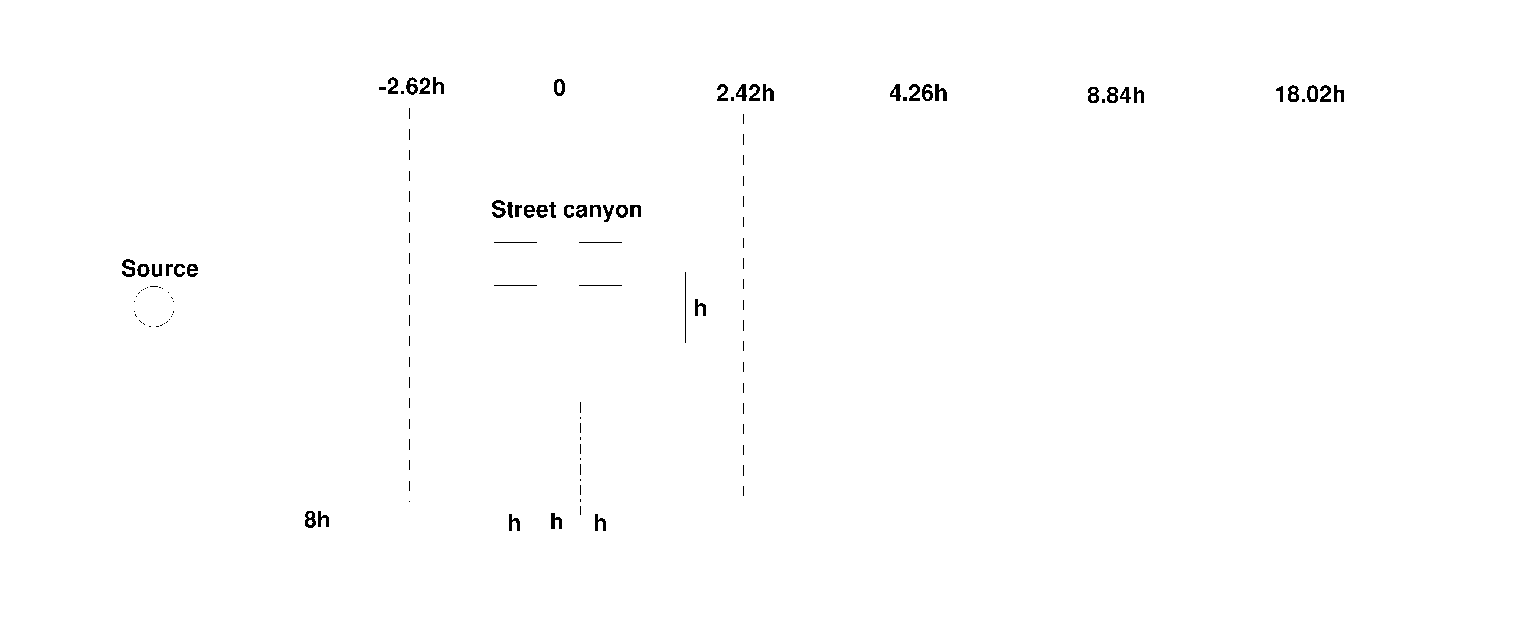
\includegraphics[width=1.1\textwidth]{Figures/layout.eps}
	\caption{Schematic overview of the domain from above. The data is collected along the dotted lines.}
	\label{fig:layout}
\end{figure}
%

Scaling the domain with the size of the boundary layer $H =1$m restricts it to
the box $0.0\leq x/H \leq 4.96,-1.75\leq y/H \leq 1.75, 0\leq z/H \leq 1.5$.
The four cubic boxes are centered around $(1.4315,0)$ with a distance $h$ between each box.
The source is placed with its center in $(0.396,0)$ and radius $r = 0.0515$.
The grid used for the computations consists of 14747 elements and with a polynomial degree of
7 the total number of nodes $N\approx 5,2$mill. 


The simulations are performed using Large Eddy Simulation (LES) 
with the dynamic Smagorinsky-Lilly subgrid-scale model and by applying the polynomial filtering
routine that is available in Nek5000. 
The release of gas will result in a plume that is advected with the wind field,
see \fref{fig:plume}. The concentration of the released gas at the 
indicated positions in \fref{fig:layout} are compared with 
experimental data and simulations performed in CDP~\cite{CDP}. 
For clarification some of the variables repeatedly mentioned throughout this thesis will be 
stated explicitly in \tref{tab:simplevariables}.
\begin{table}
    \centering
    \begin{tabular}{c c c c}
        Variable & value & unit & commentary \\ \hline
        $H$   & $1$ & m & length scale of the domain \\ 
        $h$   & $0.109$ & m & the sides of the cubic boxes\\ 
        $Q$   & $50$ & dm$^3$/min & gas release from source \\ 
        $U_{ref} $& $\approx1.08$ & m/s & reference value of $U$ \\
    \end{tabular}
    \caption{Essential variables, $U_{ref}$ is calculated as a time average of the velocity in 
        x-direction at a point far away from the floor and walls and will therefore 
        vary by a small amount from case to case. }
    \label{tab:simplevariables}
\end{table}

The inflow conditions had to be extrapolated onto the domain at each time step. To mimic the situation in the wind-tunnel the velocity field
on the inflow was generated in a different simulation performed in CDP. The inflow velocity was written to file every 
$0.0013$s for a total of $28$s and had to be interpolated onto the domain for the simulations in Nek5000 since the grid was not identical.
The right plot in \fref{fig:inflow} is an instantaneous picture of the inflow velocity in x-direction, 
notice how the pattern repeats itself along the y-axis. This is because the inflow data was generated in a smaller channel, approximately $1/3$ of the 
width of the computational domain used for the data sampling. An interpolation algorithm implemented at FFI was applied to adjust 
the inflow-data to the computational mesh, this was done directly in \verb|.usr|. 
%
\begin{figure}
\centering
  \centerline{
\begin{minipage}{.6\textwidth}
  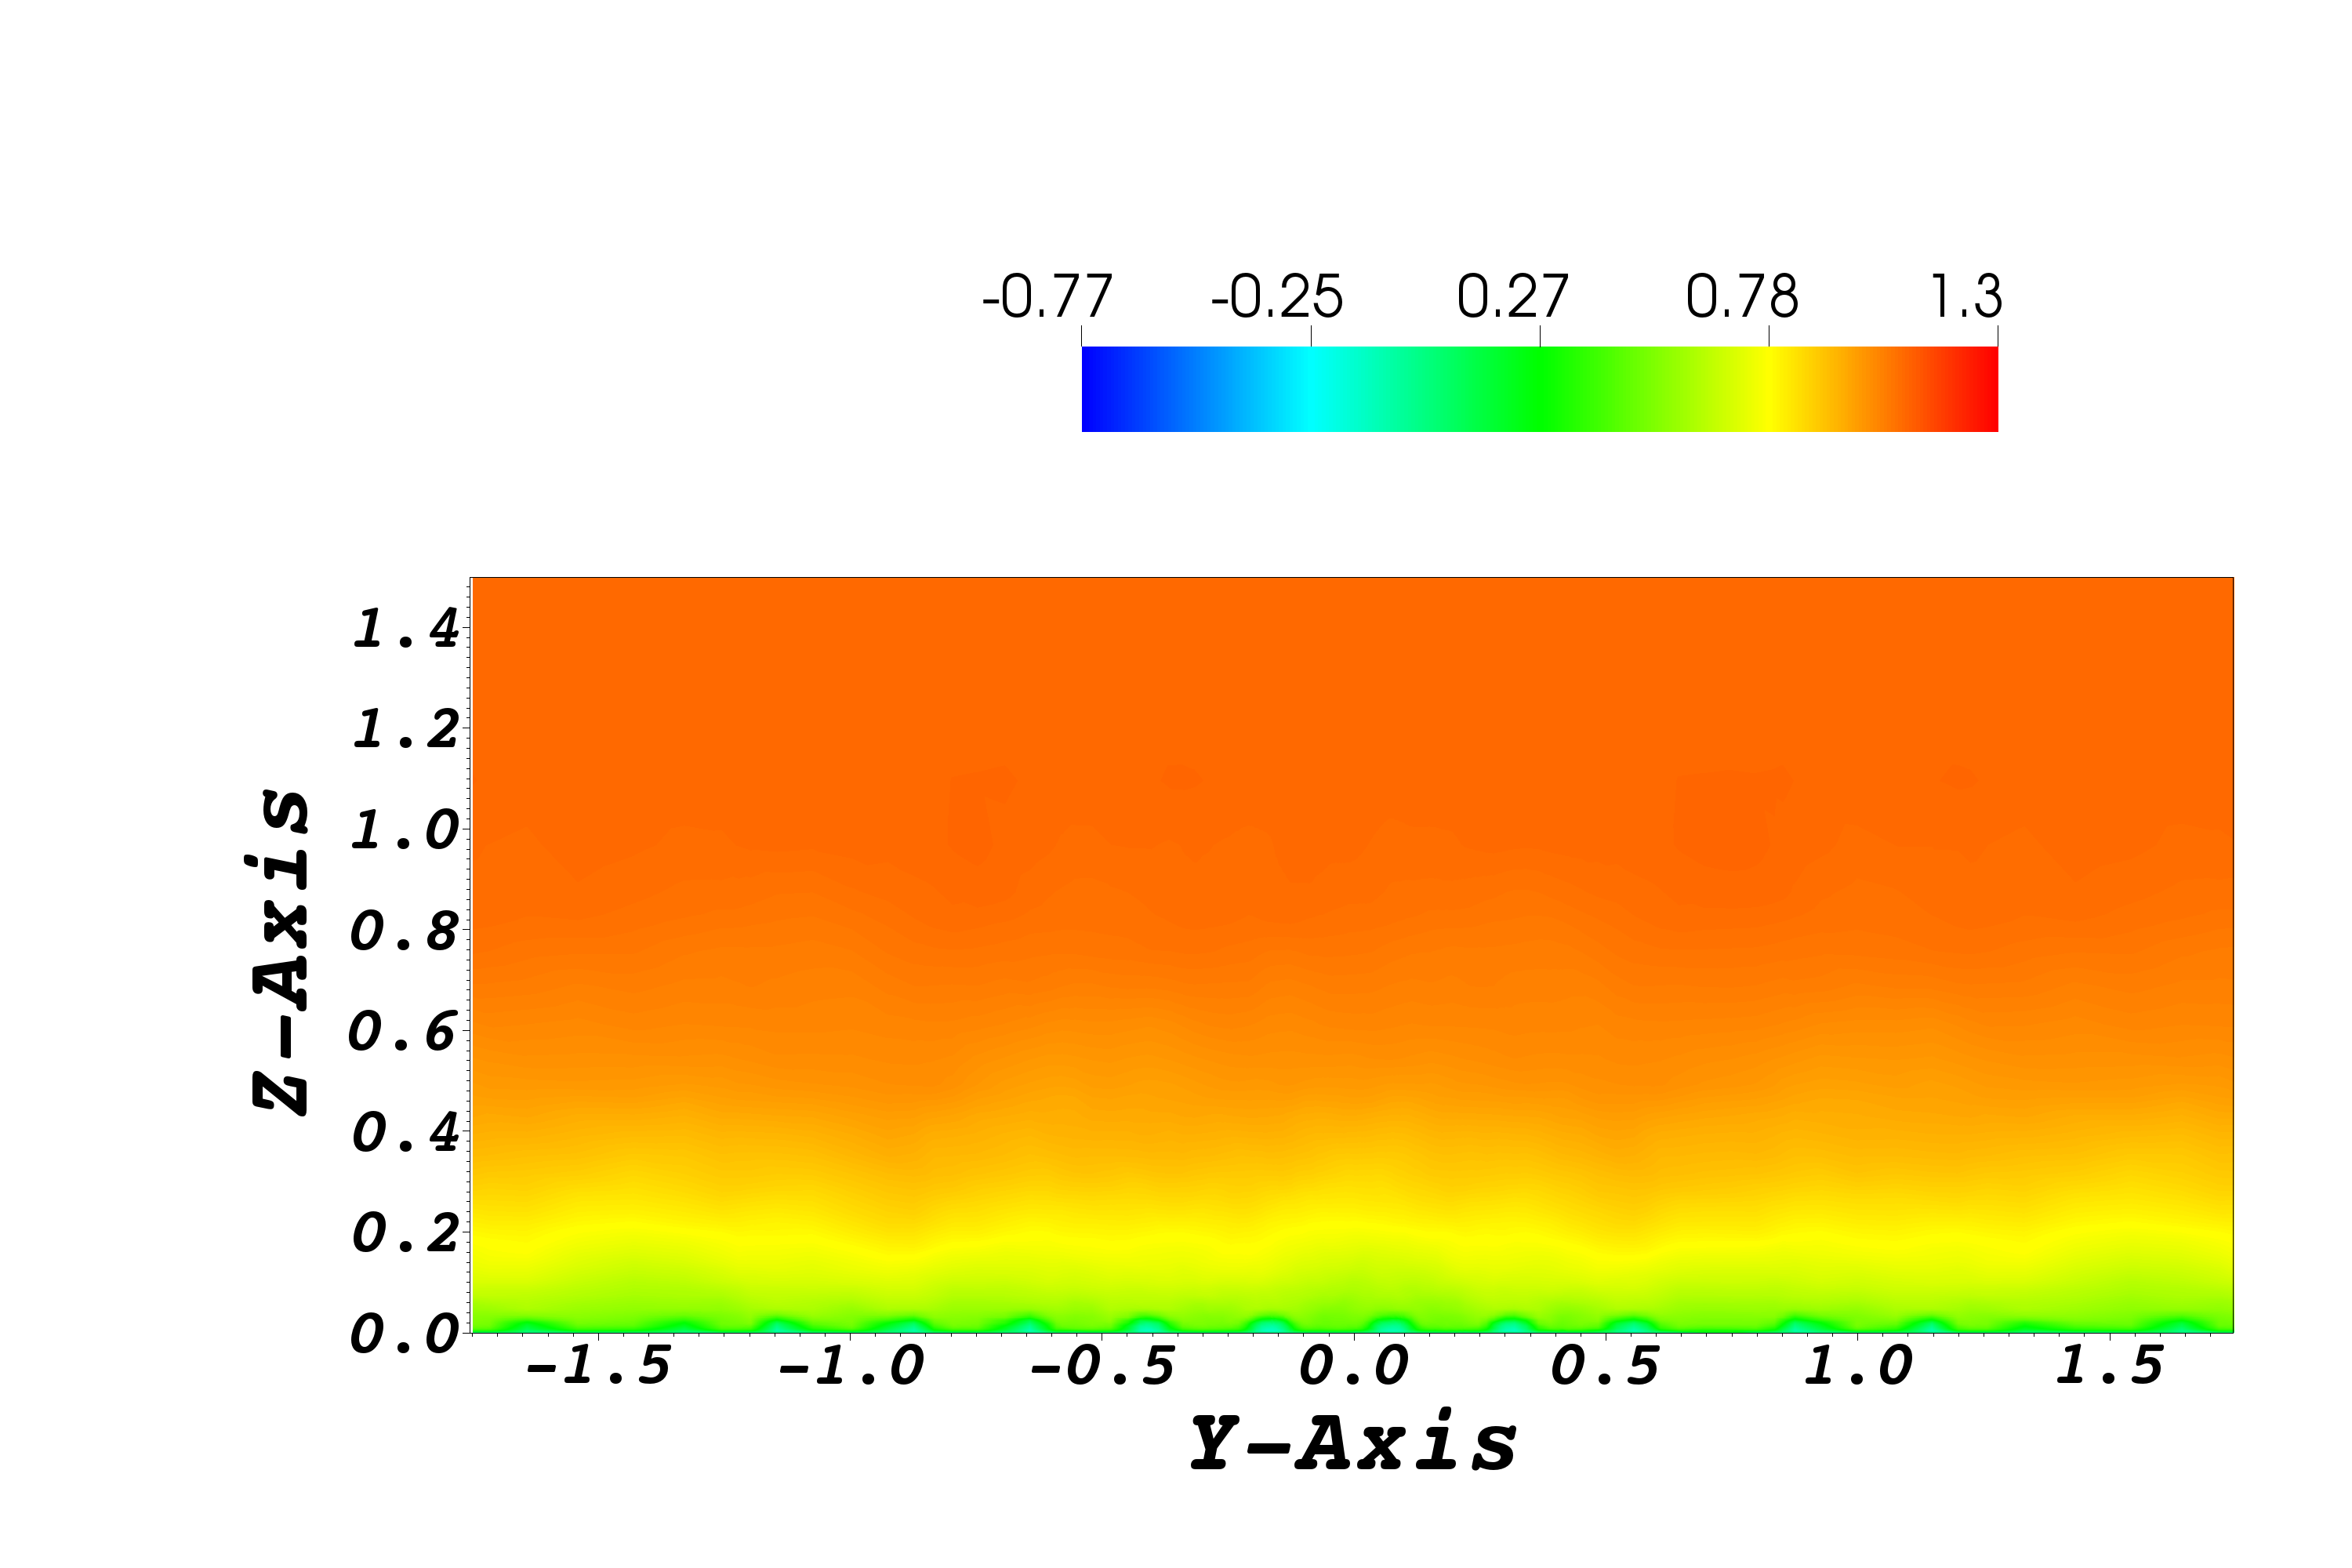
\includegraphics[width=1.0\linewidth]{Figures/inflow_field_avg.png}
  %\captionof{figure}{A figure}
\end{minipage}%
\begin{minipage}{.6\textwidth}
  \centering
  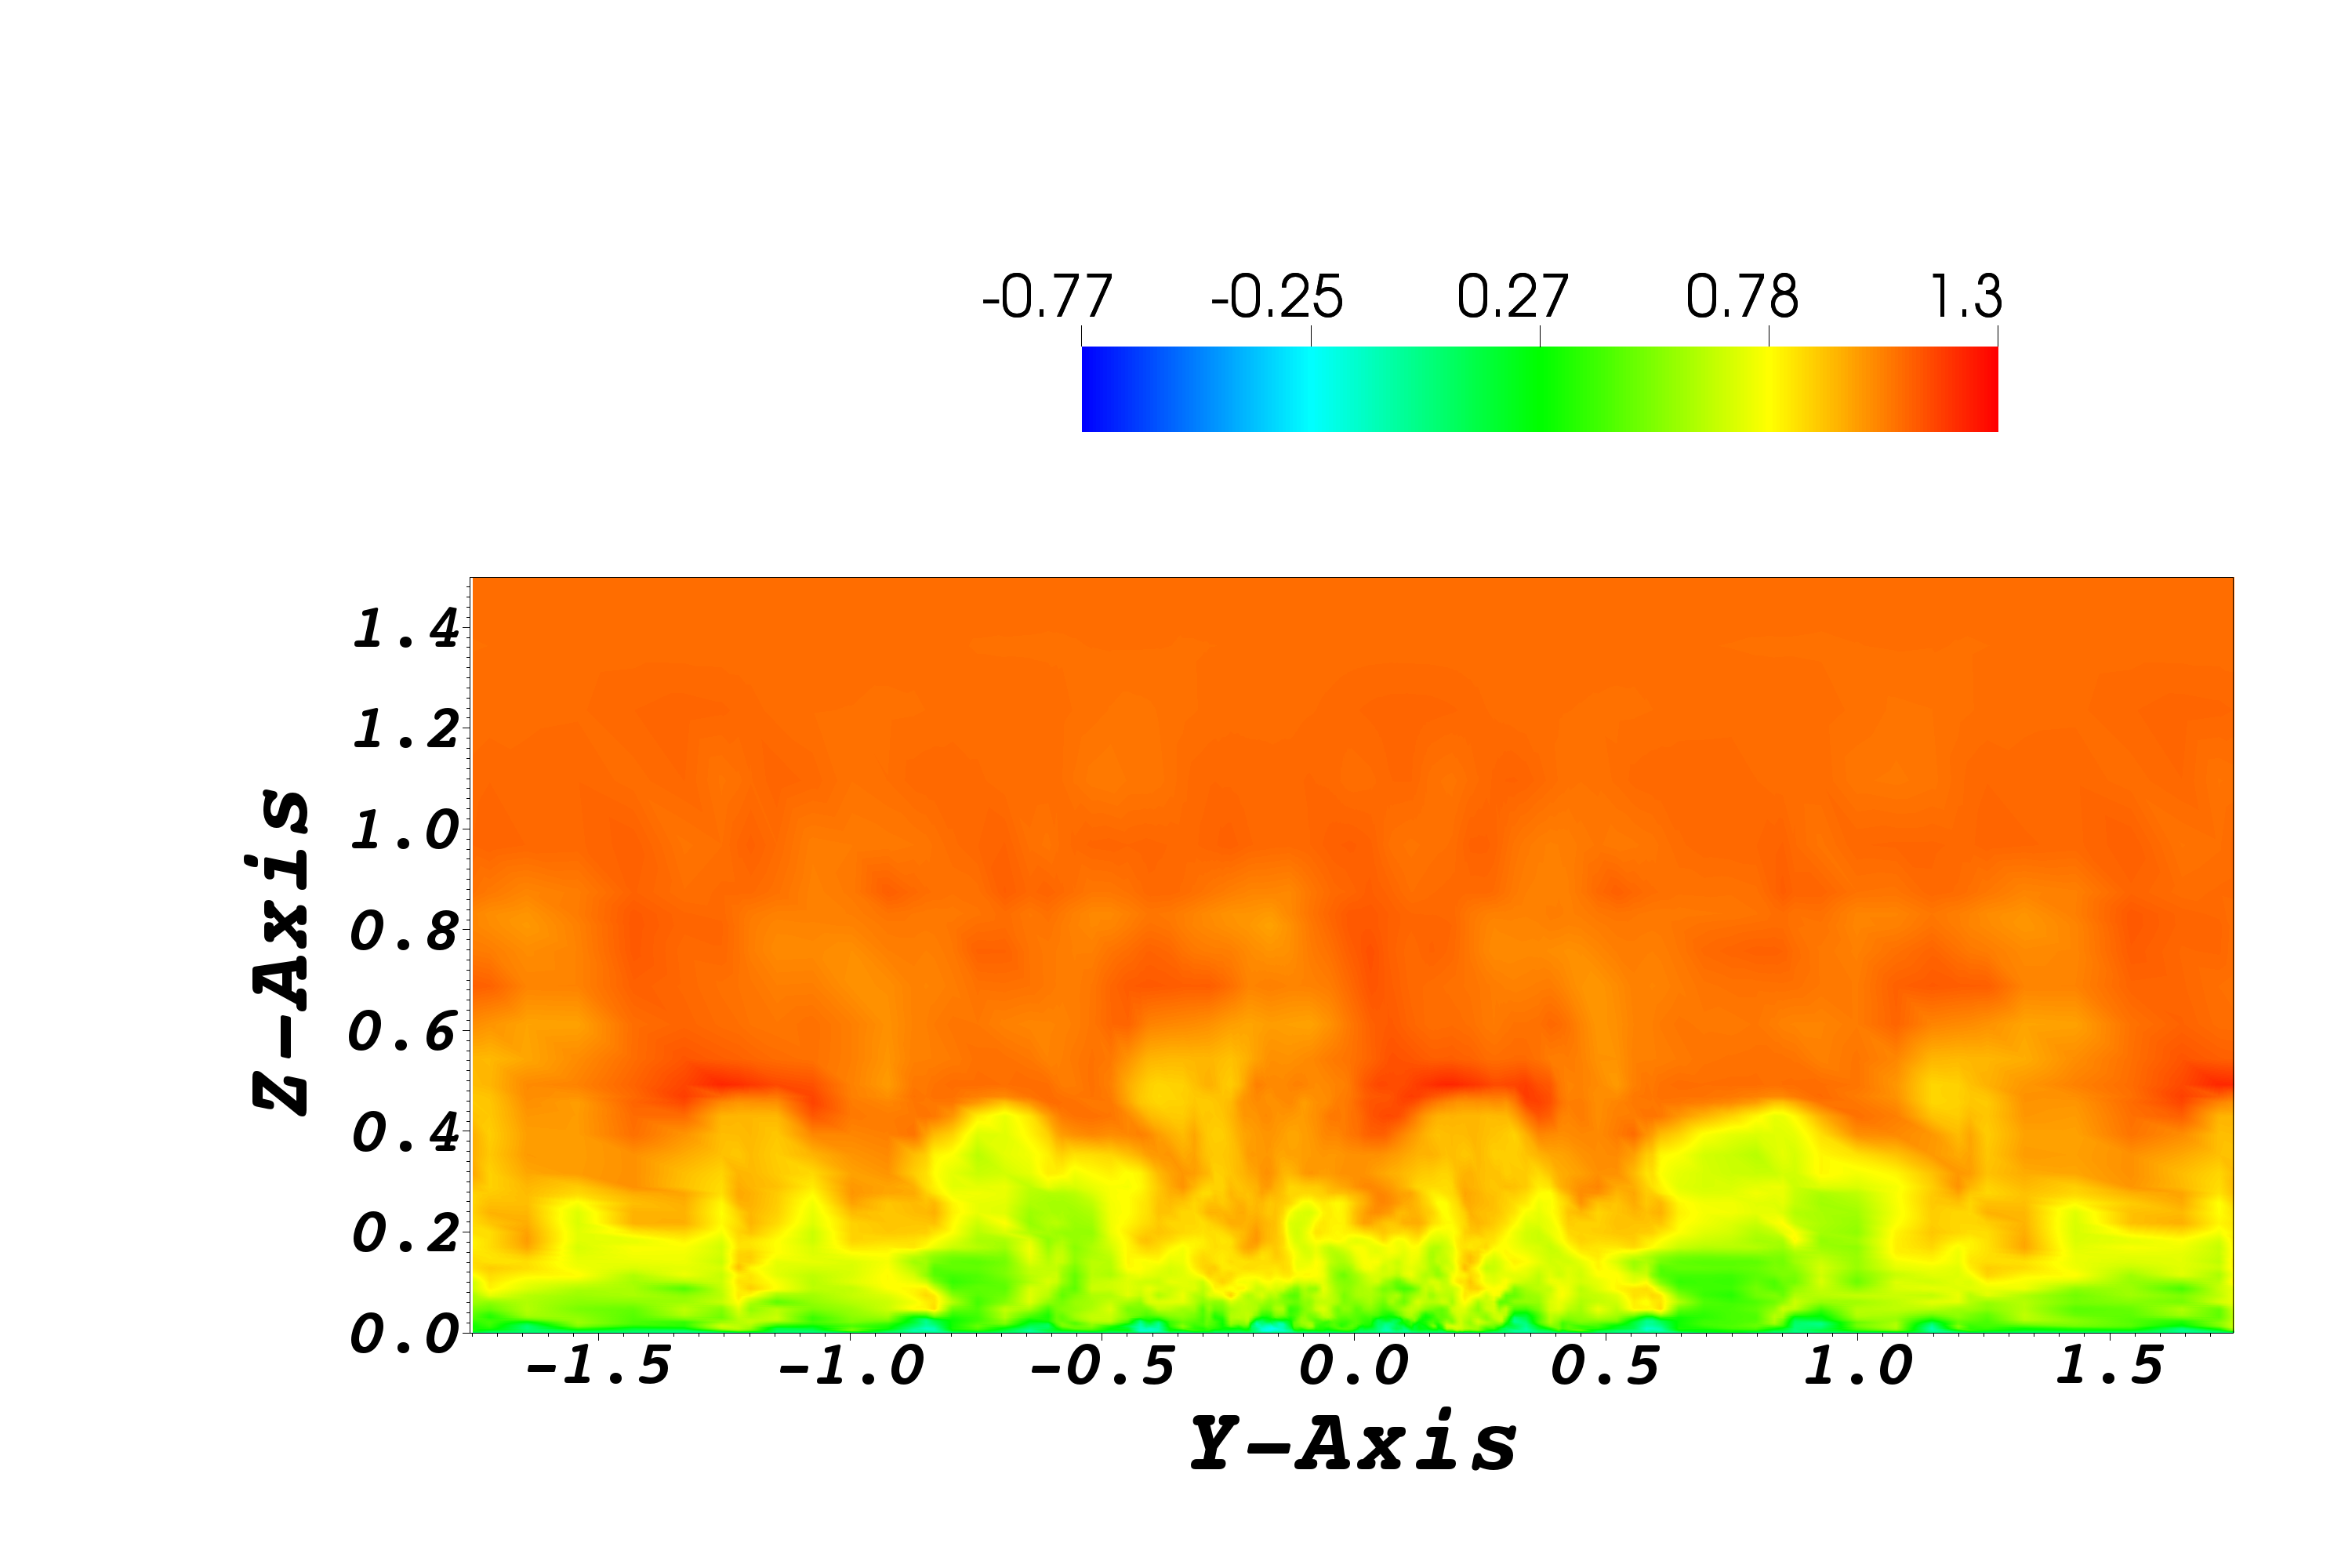
\includegraphics[width=1.0\linewidth]{Figures/inflow_field.png}
\end{minipage}
}
  \caption{The averaged (left) and instantaneous (right) x-velocity on the inflow boundary.}
  \label{fig:inflow}
\end{figure}
%

The simulations in Nek5000 were performed in the following manner; first 6 seconds of initialization of the velocity field in the 
channel, followed by 8 seconds of gas release to initialize the gas-concentration. After assuring that the wind-field was 
correctly created and the released gas had reached the measurement lines furthest from the source the data sampling of 22 seconds 
started.
%
\begin{figure}[h]
	\centering
	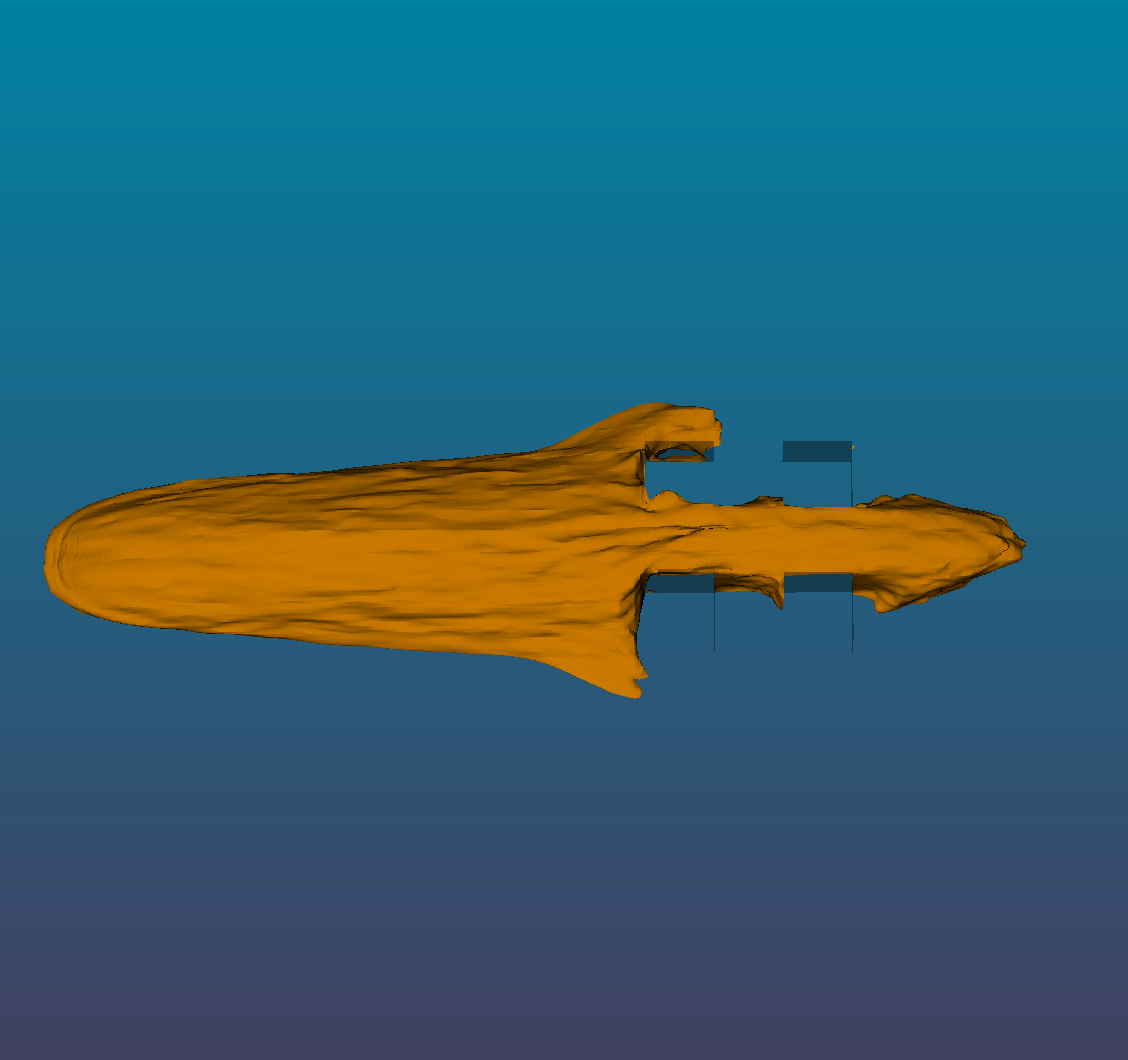
\includegraphics[width=0.6\textwidth]{Figures/plume2.png}
	\caption{An iso-surface of the average concentration with $C=0.03$ 
    after 30 seconds of sampling.}
	\label{fig:plume}
\end{figure}
%

The mesh used in the simulations performed in Nek5000 and the one performed in CDP are 
different, and the resolution in the part of the domain close to the cubes is described 
in~\tref{tab:meshdiff}.
\begin{table}
    \centering
    \begin{tabular}{c| c c c}
        Solver   & $n_x$& $n_y$ & $n_z$ \\ \hline
        CDP      & 28 & 28 & 64 \\ 
        Nek5000  & 22 & 22 & 36 
    \end{tabular}
    \caption{Number of nodes used to represent one cube.}
    \label{tab:meshdiff}
\end{table}

The resolution is better in the simulations done in CDP and especially in 
the $z$-direction. 

\subsection{Results - Gas dispersion} 
This case is a part of a larger project designed to evaluate different solvers 
ability to perform simulations of gas dispersion. The N-S equations are solved using
the $P_NP_N$ formulation with the fractional step method, IOFS with a target Courant number 
equal 2 was enabled to maximize the time step as recommended in~\cite{Nek}. It should be 
mentioned that the stability properties when activating the SGS-model and deactivating the 
filtering was greatly reduced. This effect is captured in~\fref{fig:maxvel} that shows how 
the Smagorinsky model does not damp spurious velocity modes in the same degree as the filter. 
%
\begin{figure}[h]
	\centering
	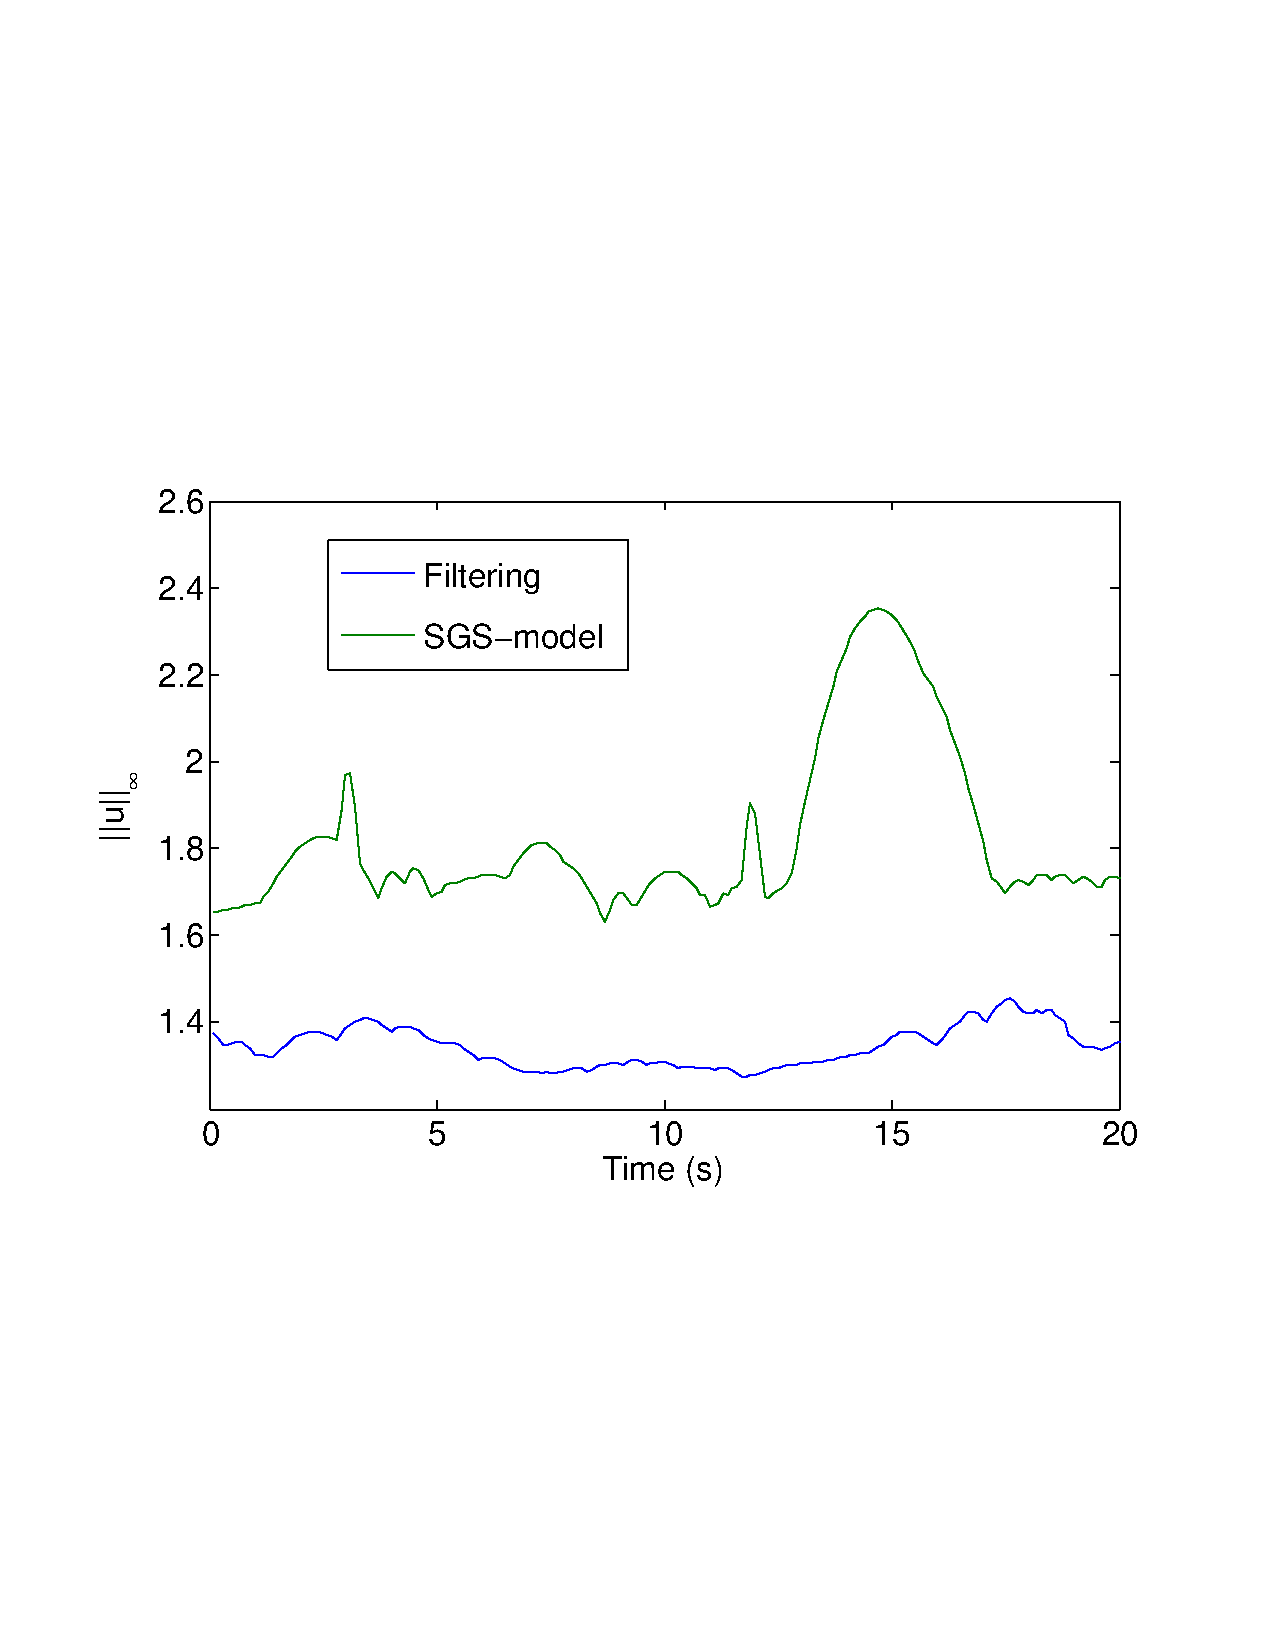
\includegraphics[trim=0.5cm 7cm 0.5cm 7cm, width=0.8\textwidth]{Figures/maxvel.pdf}
    \caption{$||\mathbf{u}||_{\infty}$ as a function of time, the green line represents the 
simulation with the dynamic Smagorinsky SGS-model and the blue line represents the filtering 
with $\alpha = 0.05$ and a quadratic decay on the last 3 modes.}
	\label{fig:maxvel}
\end{figure}
%
%
%\begin{figure}[h]
	%\centering
	%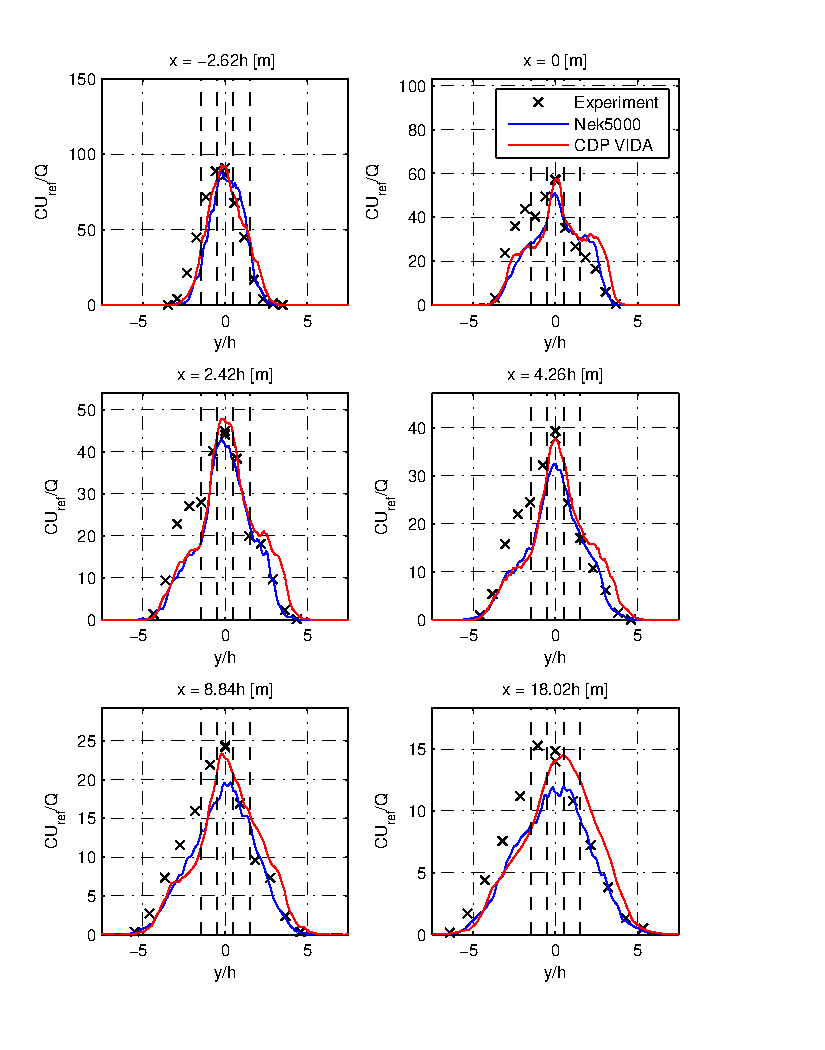
\includegraphics[width=0.8\textwidth]{Figures/NekcH.pdf}
	%\caption{Time-averaged concentration with a sample time of $18.00$ s at $z/H = 0.025$ plotted horizontally and scaled 
	%with the free-stream velocity and emission rate. Compared against wind tunnel data.
%Two dashed lines on either side of the centerline represent the canyon.}
	%\label{fig:cHfilter}
%\end{figure}
%
%
%\begin{figure}[h]
	%\centerline{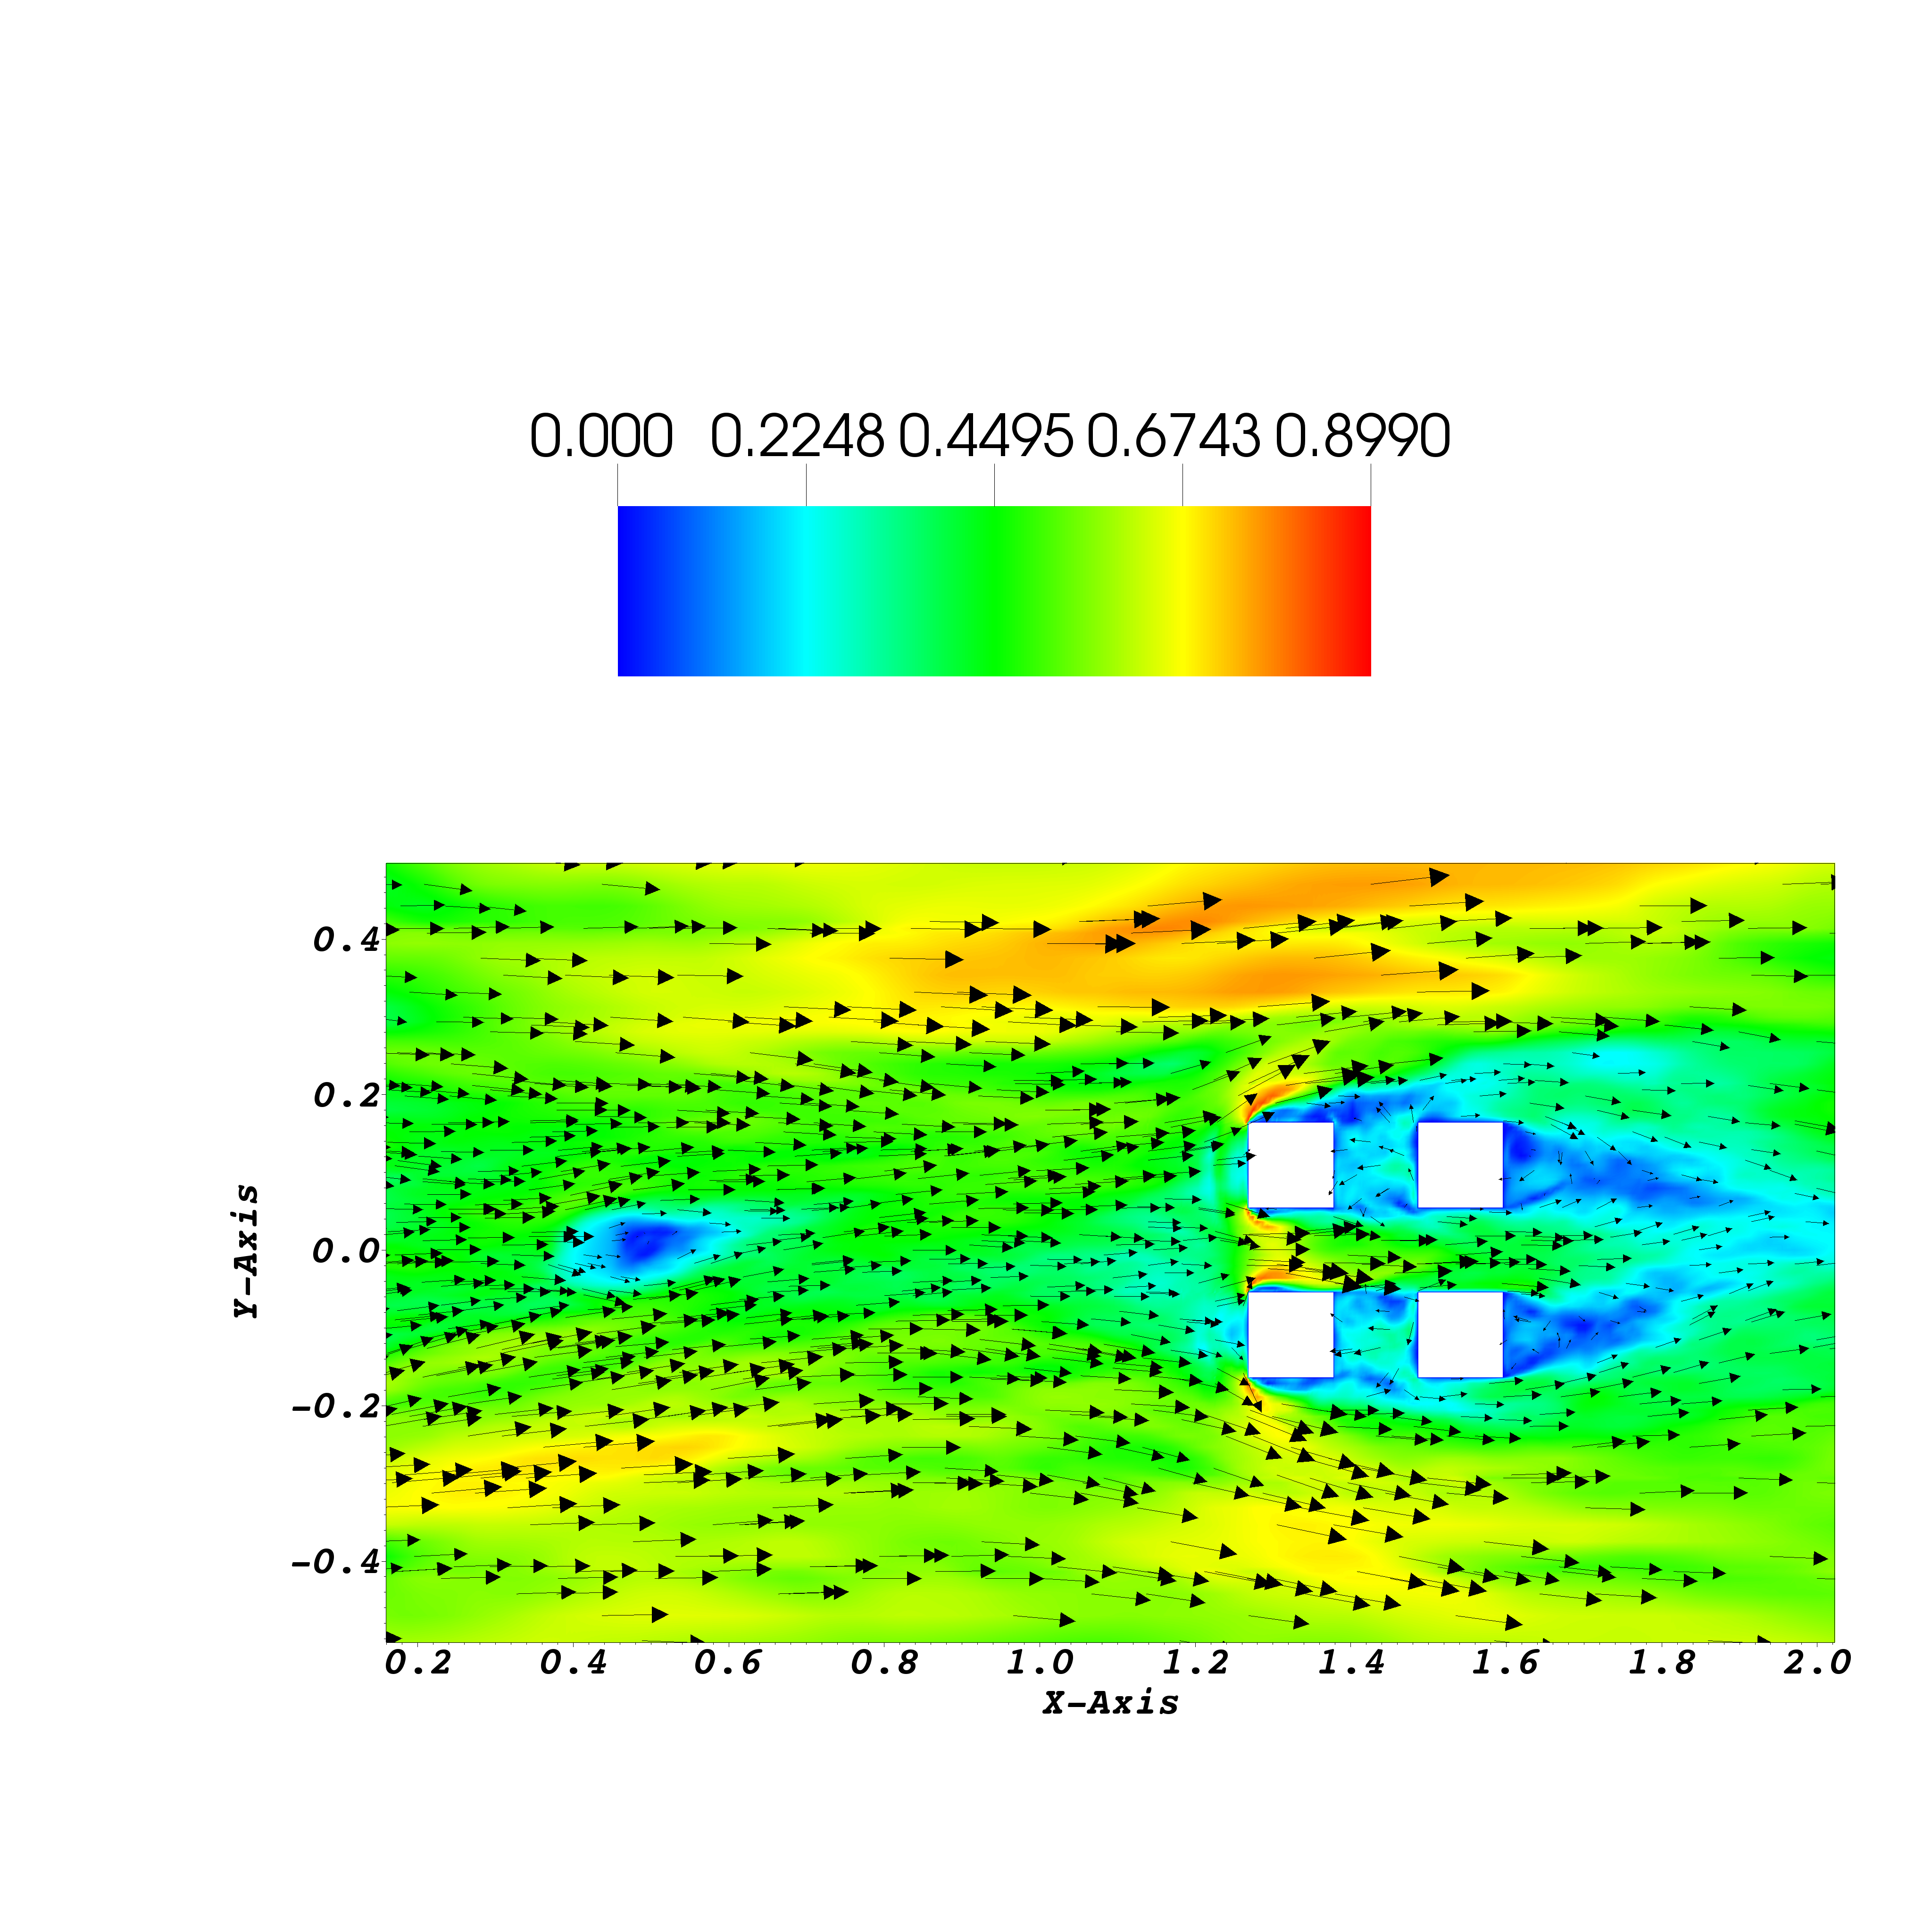
\includegraphics[width=0.8\textwidth]{Figures/vel_field.png}}
	%\caption{velocity field for $z= 0.02$m, around the source and the cubes.}
	%\label{fig:vel_field}
%\end{figure}
%

%\colorbox{green}{redo these simulation in case they were started to early.}
%
%\begin{figure}[h]
	%\centering
	%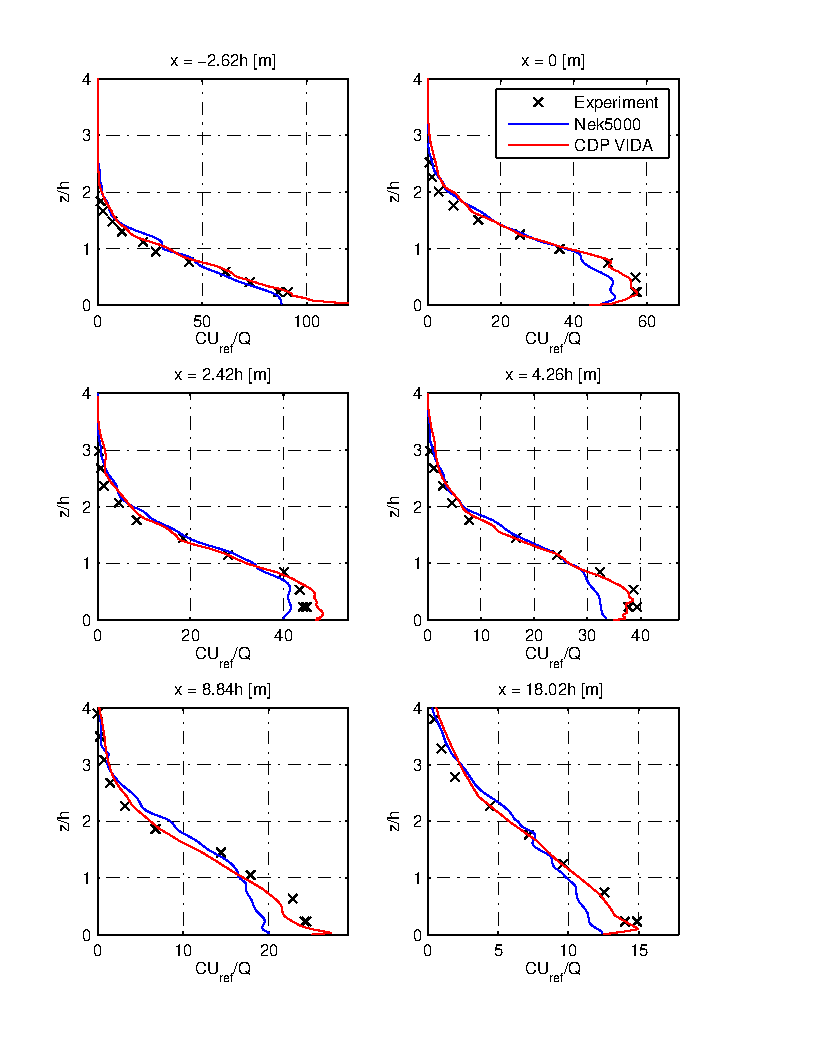
\includegraphics[width=0.8\textwidth]{Figures/NekcV.pdf}
	%\caption{Time-averaged concentration with a sample time of $18.00$ s at $y = 0$ plotted
    %vertically and scaled 
	%with the free-stream velocity and emission rate. Compared against wind tunnel data.
%Two dashed lines on either side of the centerline represent the canyon.}
	%\label{fig:cVfilter}
%\end{figure}
%
%
%\begin{figure}[h]
	%\centering
	%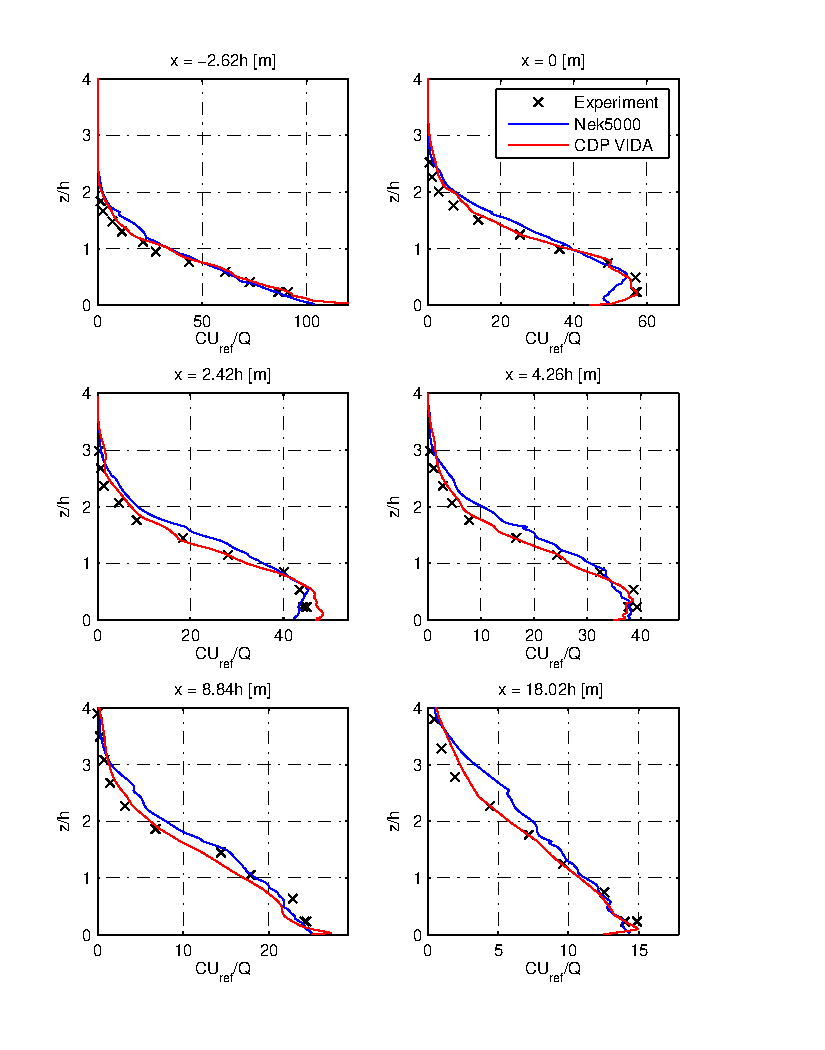
\includegraphics[width=0.8\textwidth]{Figures/Nek_smag_cV.pdf}
	%\caption{Time-averaged concentration with a sample time of $22.00$ s at $y = 0$ plotted
    %vertically and scaled 
	%with the free-stream velocity and emission rate. Compared against wind tunnel data.
%Two dashed lines on either side of the centerline represent the canyon.}
	%\label{fig:cVsmag}
%\end{figure}
%
%
%\begin{figure}[h]
	%\centering
	%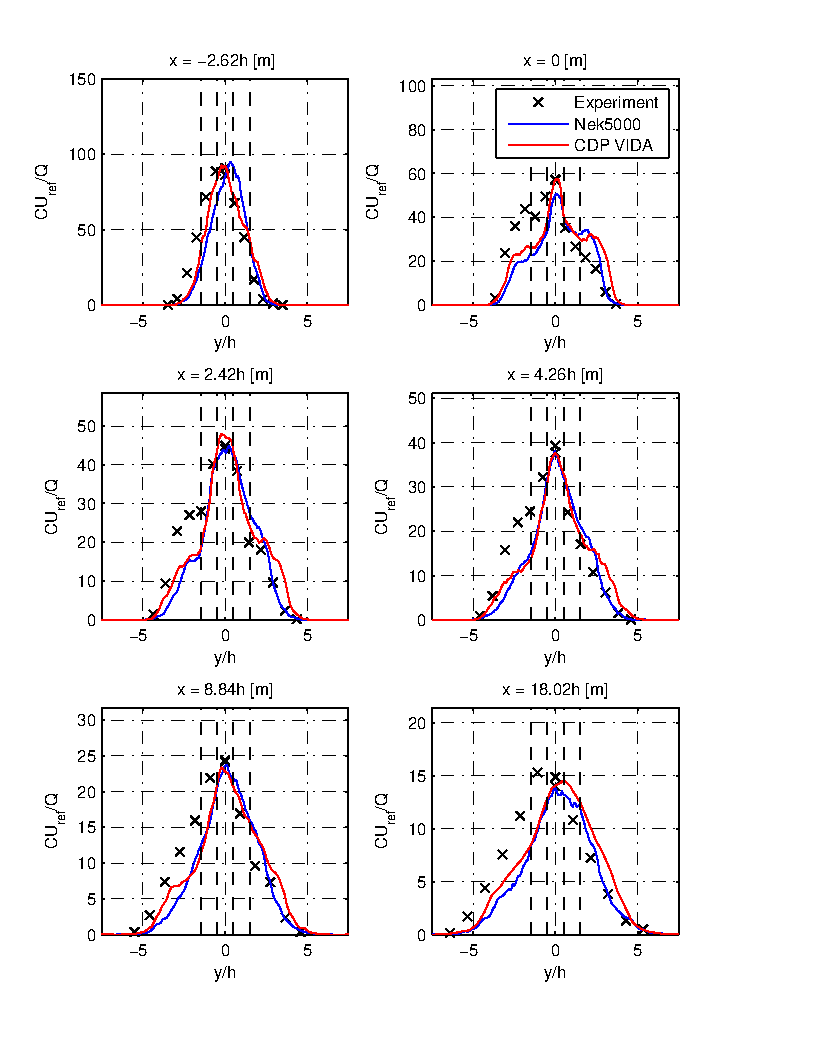
\includegraphics[width=0.8\textwidth]{Figures/Nek_smag_cH.pdf}
	%\caption{Time-averaged concentration with a sample time of $22.00$ s at $y = 0$ plotted
    %vertically and scaled 
	%with the free-stream velocity and emission rate. Compared against wind tunnel data.
%Two dashed lines on either side of the centerline represent the canyon.}
	%\label{fig:cVsmag}
%\end{figure}
%
\newpage
\begin{figure}[h]
    \centering
    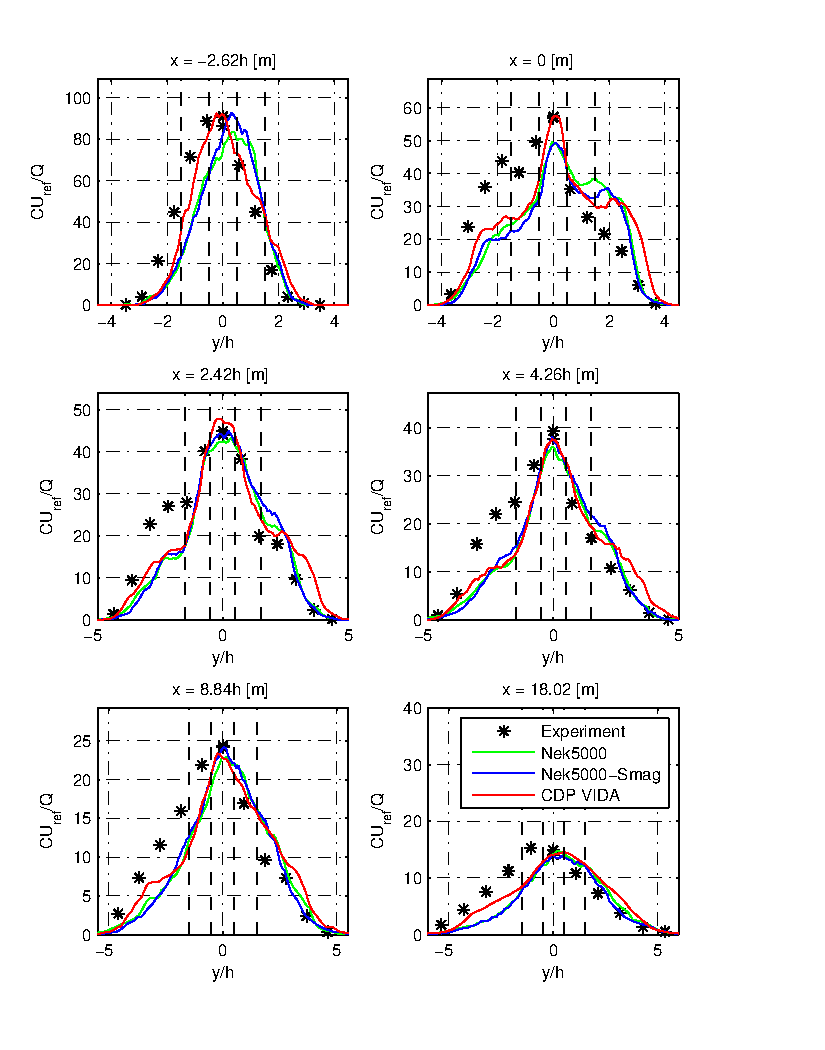
\includegraphics[width=0.9\textwidth]{Figures/NekcH_all.pdf}
    \caption{Time-averaged concentration with a sample time of $22.00$ s at $y = 0$ plotted
    vertically and scaled 
    with the free-stream velocity and emission rate. Compared against wind tunnel data.
Two dashed lines on either side of the centerline represent the canyon.}
    \label{fig:cHall}
\end{figure}

\fref{fig:cHall} shows the scaled concentration along the dotted lines in~\fref{fig:layout}. 
According to this figure Nek5000 does indeed capture the important features of the mean concentration.
At the two first measurement lines the results are slightly skewed to the right, this is to some degree 
also the case for the CDP simulations but not for the experiment. A possible explanation could be that 
the inflow condition favours one of the sides of the domain, or simply that the sampling time is not 
sufficiently long. 
%Along the second measurement line which is placed in the middle of the 4 cubes Nek5000 
%estimates a concentration peak lower than both the reference solutions.  

The results also indicate that the difference between the SGS-model and the filtering
is not that large,
if anything the SGS-model shows a tendency to estimate higher concentration peaks.
In particular the first plot indicates a significant difference.
An important difference between the filtering and the SGS-model is 
that the filter works based on the current state of the flow 
whereas the amount of diffusion added by the SGS-model is mostly decided
by the previous states of the flow.
This could lead to either too much or too little smoothening locally.

\newpage
\begin{figure}[h]
    \centering
    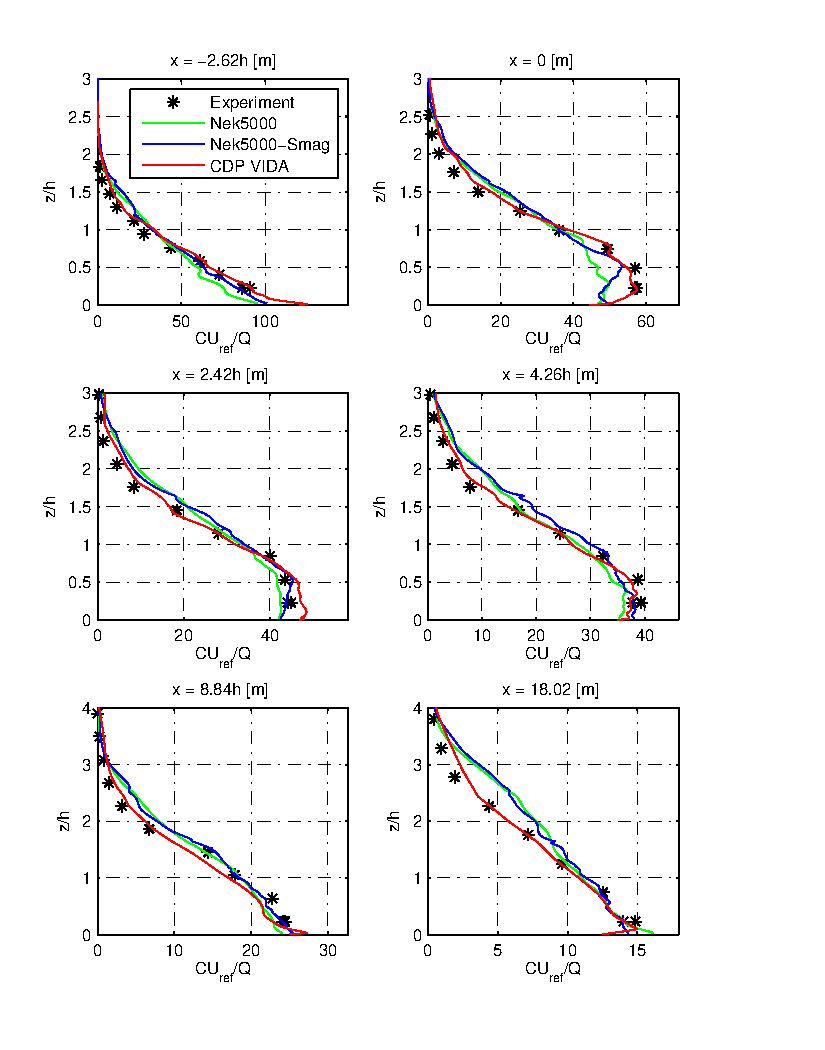
\includegraphics[width=0.9\textwidth]{Figures/NekcV_all.pdf}
    \caption{Time-averaged concentration with a sample time of $22.00$ s at $y = 0$ plotted
    vertically and scaled 
    with the free-stream velocity and emission rate. Compared against wind tunnel data.
Two dashed lines on either side of the centerline represent the canyon.}
    \label{fig:cVall}
\end{figure}
The concentration along the vertical measurement lines is plotted in \fref{fig:cVall} and overall 
Nek5000 provides good results according to the reference solutions. The largest difference is found close 
to the wall right in the middle of the cubes. In particular the simulation with filtering 
underestimates the concentration in this domain. The resolution of the mesh used for the 
Nek5000 simulations in this area is notably worse than for the CDP-simulations.
And in the middle of the cubes neither one of the filter or the Dynamic Smagorinsky model
are able to correct this.
The $P_NP_N$ formulation is known to produce splitting errors of significant sizes 
close to the wall, and could play an important role in this part of the domain.

The simulations were also performed using the $P_NP_{N-2}$ formulation with filtering, and the 
results were similar to those observed above. The SGS-model did however not function at all, 
and resulted in a system crash in one of the earliest time-steps.

As for the performance of Nek5000 the results are baffling. With the same number of processors,
same accuracy criteria, and approximately the same number of nodes in the grid, Nek5000 simulated
one second of flow more than five times as fast as a numerical code comparable to CDP! 
This was done without any particular tuning and with a time-step about $2/3$ of the one used in 
CDP. 


%\begin{figure}[h]
    %\centering
    %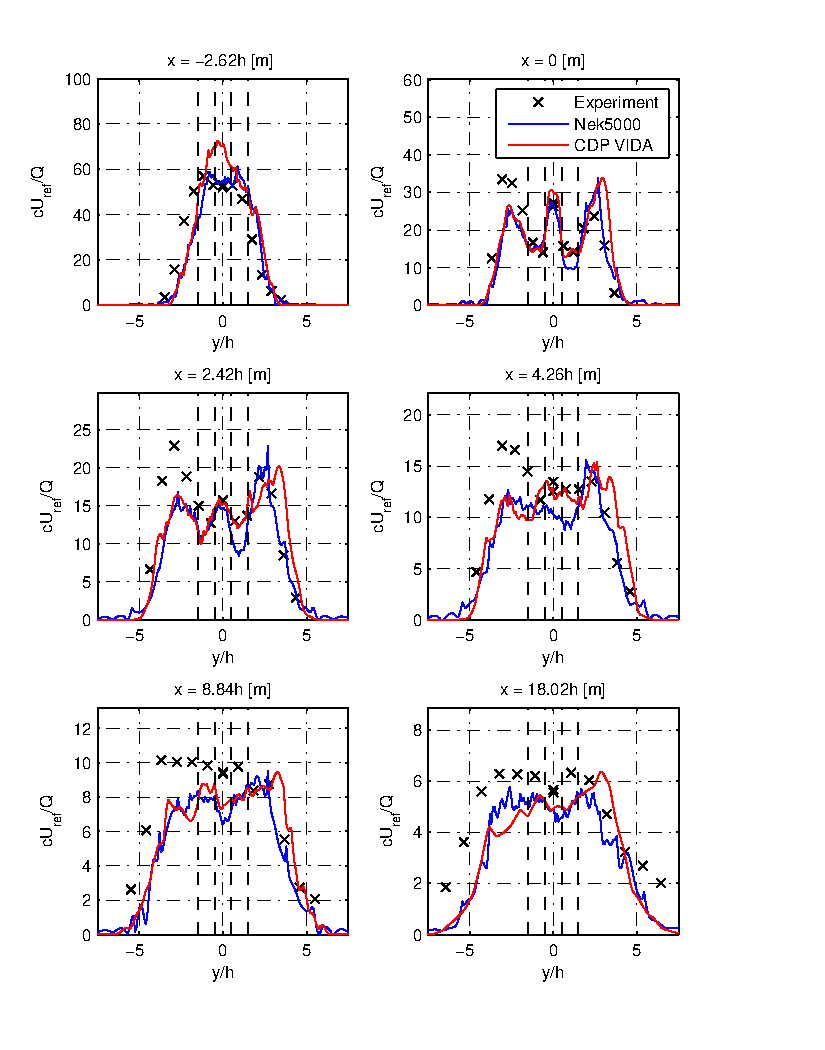
\includegraphics[width=0.8\textwidth]{Figures/Nek_smag_cfluctH.pdf}
    %\caption{Time-averaged concentration with a sample time of $22.00$ s at $y = 0$ plotted
    %vertically and scaled 
    %with the free-stream velocity and emission rate. Compared against wind tunnel data.
%Two dashed lines on either side of the centerline represent the canyon.}
    %\label{fig:cVsmag}
%\end{figure}


\section{Case 2: Drag and lift on a cylinder}
A standard benchmark case for flow solvers is presented in~\cite{benchmark}. 
The case is to calculate the drag and lift coefficients on a cylinder in a rectangular channel.
The setup for the domain and boundary conditions are given in \fref{fig:cylinder}.
The constants applied in the description of the geometry and the coefficient scales are listed 
in table \tref{tab:case2consts}.
%
\begin{table}[h]
    \centering
    \begin{tabular}{c l l}
     Constant & Value & Property \\ \hline
    $H$ & $0.41\text{m}$ & Width and height for the channel \\
    $D$ & $0.1\text{m}$ & Diameter of the cylinder and length scale \\
    $U$ & $0.2\text{m/s}$ & Velocity scale \\
    $\nu$ &  $ 10^{-3}\text{m$^2$/s}$ & Kinematic viscosity of the fluid \\
    $Re$ & $20$ & Reynolds number \\ 
    \end{tabular}
    \caption{Constants for case 2}
    \label{tab:case2consts}
\end{table}
%
Finding the drag and lift coefficient requires a calculation of the velocity field around the cylinder
which is done by solving the unsteady N-S equations until a steady flow is reached. This implies that the
spatial accuracy will dominate the error and one would expect great results in Nek5000 
due to its spectral convergence rate.

The flow is laminar with Reynolds number $Re=20$ so all the 
challenges arising when dealing with turbulent flow does not come to play in this case. 
%
\begin{figure}[h]
    \centering
    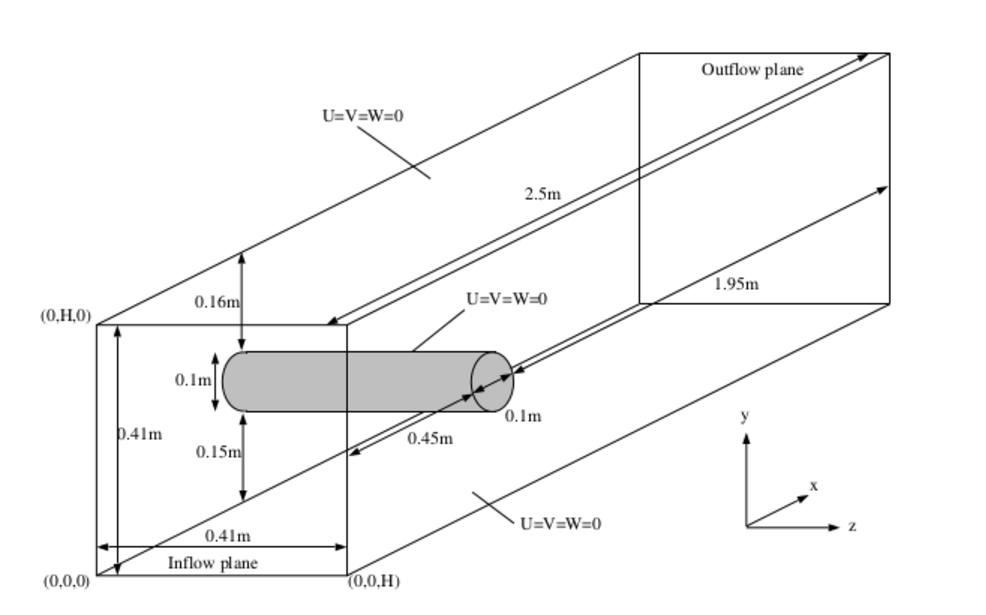
\includegraphics[width = 1.0\textwidth]{Figures/cylinder.pdf}
    \caption{Computational domain and boundary conditions.}
    \label{fig:cylinder}
\end{figure}
%
The drag and lift forces on a surface $S$ are given as 
%
\begin{align}
    F_D = \int_{S}(\rho \nu \frac{\partial v_t}{\partial n}n_y-pn_x)dS, \qquad
    F_L = -\int_{S}(\rho \nu \frac{\partial v_t}{\partial n}n_x+pn_y)dS.
    \label{eq:dragnlift}
\end{align}
%
$v_t$ is the tangential velocity, $\mathbf{n}=[n_x,n_y,0]$ is the unit vector normal to the surface $S$ 
and the tangent velocity vector is defined as $\mathbf{t} = [n_y,-n_x,0]$.
 
Surface integrals in Nek5000 are solved numerically, $\int_S f dS = \sum f_i A_i$, where $f$ is some function and $A_i$ is the area corresponding
to the nodal value $f_i$. $A_i$ corresponds to a two dimensional mass matrix in Nek5000 available for all elements.

The coefficients corresponding to these forces known as the drag and lift coefficients 
are given by the formulas 
\begin{align}
    c_D = \frac{2F_D}{\rho U^2 D H}
    \qquad , \qquad
    c_L = \frac{2F_L}{\rho U^2 D H}.
    \label{eq:dragnliftcoeffs}
\end{align}


Nek5000 provides functions for calculating lift and drag on any user-specified object.
The function is called \verb|drag_calc(scale)|, with the input parameter 
defined by the user, for this case \verb|scale| $=2/(\rho U^2DH)$.  
Apart from this the function \verb|set_obj()| has to be modified to create an object 
that consists of pointers to all the faces on the cylinder.
%Let $x,y$ be points in the computational domain, $x_c,y_c$ be the coordinates to the 
%center line in the cylinder and $0<tol\ll1$ be some user defined tolerance. The faces that belong to the cylinder can then be found by 
%looping over all elements and their faces evaluating $\epsilon = \sqrt{(x-x_c)^2+(y-y_c)}$.
%If $\epsilon < tol$ for an entire face then this face is known to 
%belong to the cylinder and is added to the object. Nek also allows the user to specify multiple objects 
%assigning the faces of interest to object 1, object 2 etc. The geometry and mesh 
%for this case was generated in ICEM, and the total number of elements are 2070. 
%For the final calculation polynomial degree $P = 11$ was applied leading to a 
%total of $N = 2755170$.
%
\begin{figure}[h]
    \centering
    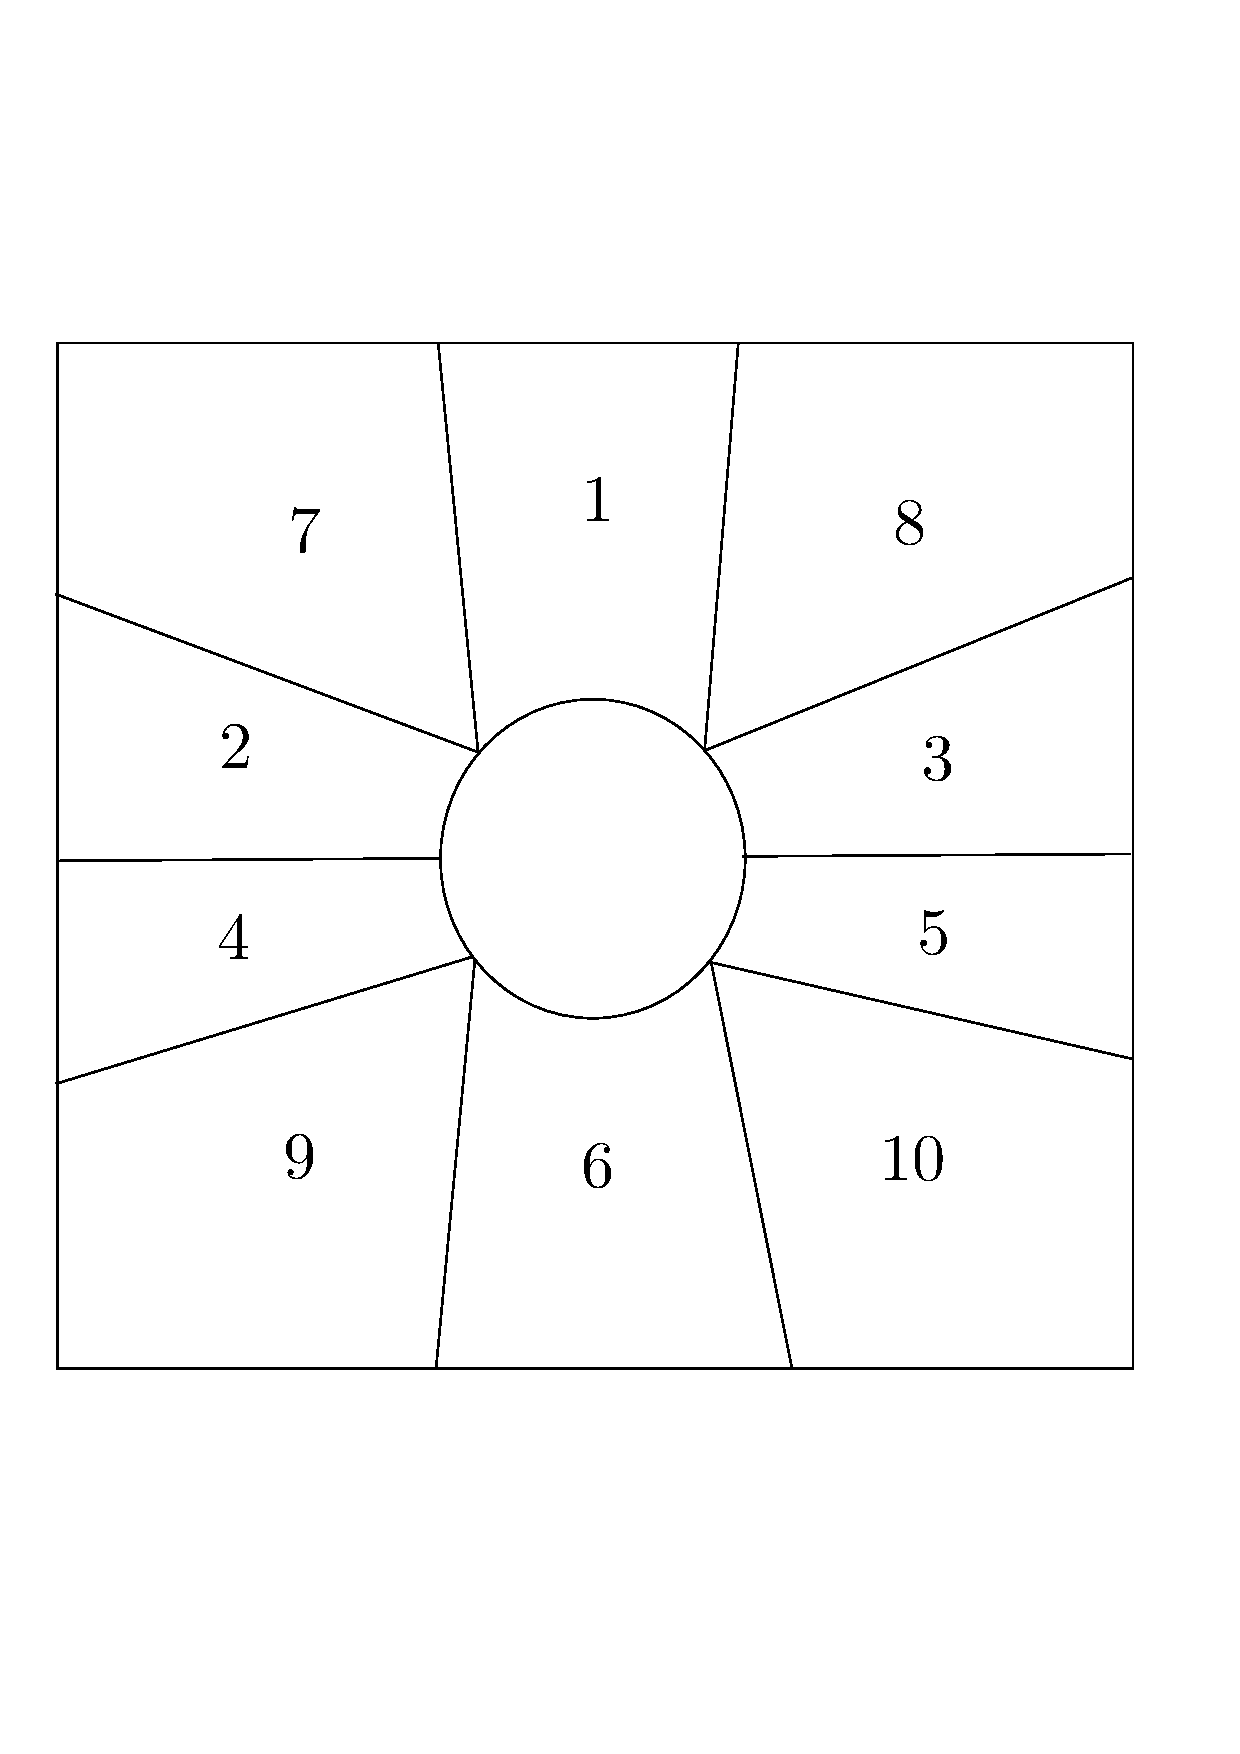
\includegraphics[width = 0.3\textwidth]{Figures/cyl_elem.pdf}
    \caption{Initial mesh around cylinder.}
    \label{fig:cyl_elem}
\end{figure}
%
The mesh around the cylinder is illustrated in \fref{fig:cyl_elem}.
Initially this case was solved using a second degree polynomial to describe the circle segments
corresponding to each element. However with the new routine implemented as described 
in~\cref{xyzarc} the circle segments could be represented with the same order as 
the polynomials used for the velocity space. The importance of the error resulting 
from the second degree approximation of the circle segments is presented in \cref{results}.
%Note that these elements was split in three, in order to obtain 
%a finer mesh in the region of interest. Of the elements numbered in~\fref{fig:cyl_elem}
%only the first six contains edges on the cylinder.Hence the second order polynomials 
%describing the curved edges describe approximately $\Theta = 360^{\circ}/(6\cdot 3) = 20^{\circ}$
%of the complete circle. 

An additional test that is performed on this case is how different settings in Nek5000 will affect the estimation of the drag and lift coefficients.
Perhaps most curious is whether the $P_NP_N$ or $P_NP_{N-2}$ formulation is applied. Note that the pressure in the latter formulation is 
not defined on the boundary of the cylinder and does therefore need to be extrapolated onto the surface in order for the integral to be 
calculated. On the other side is the splitting scheme implied by the $P_NP_N$ forces the erroneous boundary condition on the pressure.
%
\subsection{Results - benchmark comparison}
The effect of the algorithm explained in \cref{xyzarc} is
illustrated by solving a laminar flow test problem. 
The solution is compared with previously benchmark computations performed by a number of 
contributors~\cite{benchmark}. 

The results are presented in \tref{tab:testcase}, and they confirm that the treatment of the geometry is 
essential, both coefficients are computed with significantly better accuracy. 
%
\begin{table}[h]
\centering
\begin{tabular}{l l c c c c}
		\toprule
		\# of Cells & Software & $c_D$ & $c_L$ & \%\textbf{Err} $c_D$ &\%\textbf{Err} $c_L$ \\ \midrule 
		2124030& Nek5000 (mid) & 6.18349 & 0.008939 & 0.030 & 4.19 \\ 
		2124030& Nek5000 (arc) & 6.18498 & 0.009413 & 0.006 & 0.13 \\
		3145728 & CFX 		 & 6.18287 & 0.009387 & 0.04 &0.15 \\
		3145728 & OF	     & 6.18931 & 0.00973 & 0.06 &3.5 \\
		3145728 & FEATFLOW   & 6.18465 & 0.009397 & 0.01 &0.05 \\
		\bottomrule	
	\end{tabular}
	\caption{Results for the drag and lift coefficients with reference values 
	$c_D = 6.18533$ and $c_L = 0.009401$. $p=11$ for the simulations in Nek5000.}
\label{tab:testcase}
\end{table}
%
Compared with the results from the other softwares applied in~\cite{benchmark} Nek5000 performs 
just as well or better in most cases. It should be mentioned that the division of the grid is created
in a different manner for Nek5000 so the comparison is not as direct as it may seem from the table.

\subsection{Results - internal adjustments }
As discussed in \cref{nek} there are many adjustments available in Nek5000. 
To enlighten the actual effect on the results, several different settings were 
investigated for this case and the results are presented in \tref{tab:perf}. 
The spectral convergence is also confirmed in \fref{fig:liftconv} by calculating the 
lift coefficient error for increasing polynomial degree. 
%
\begin{figure}[h]
	\centerline{
        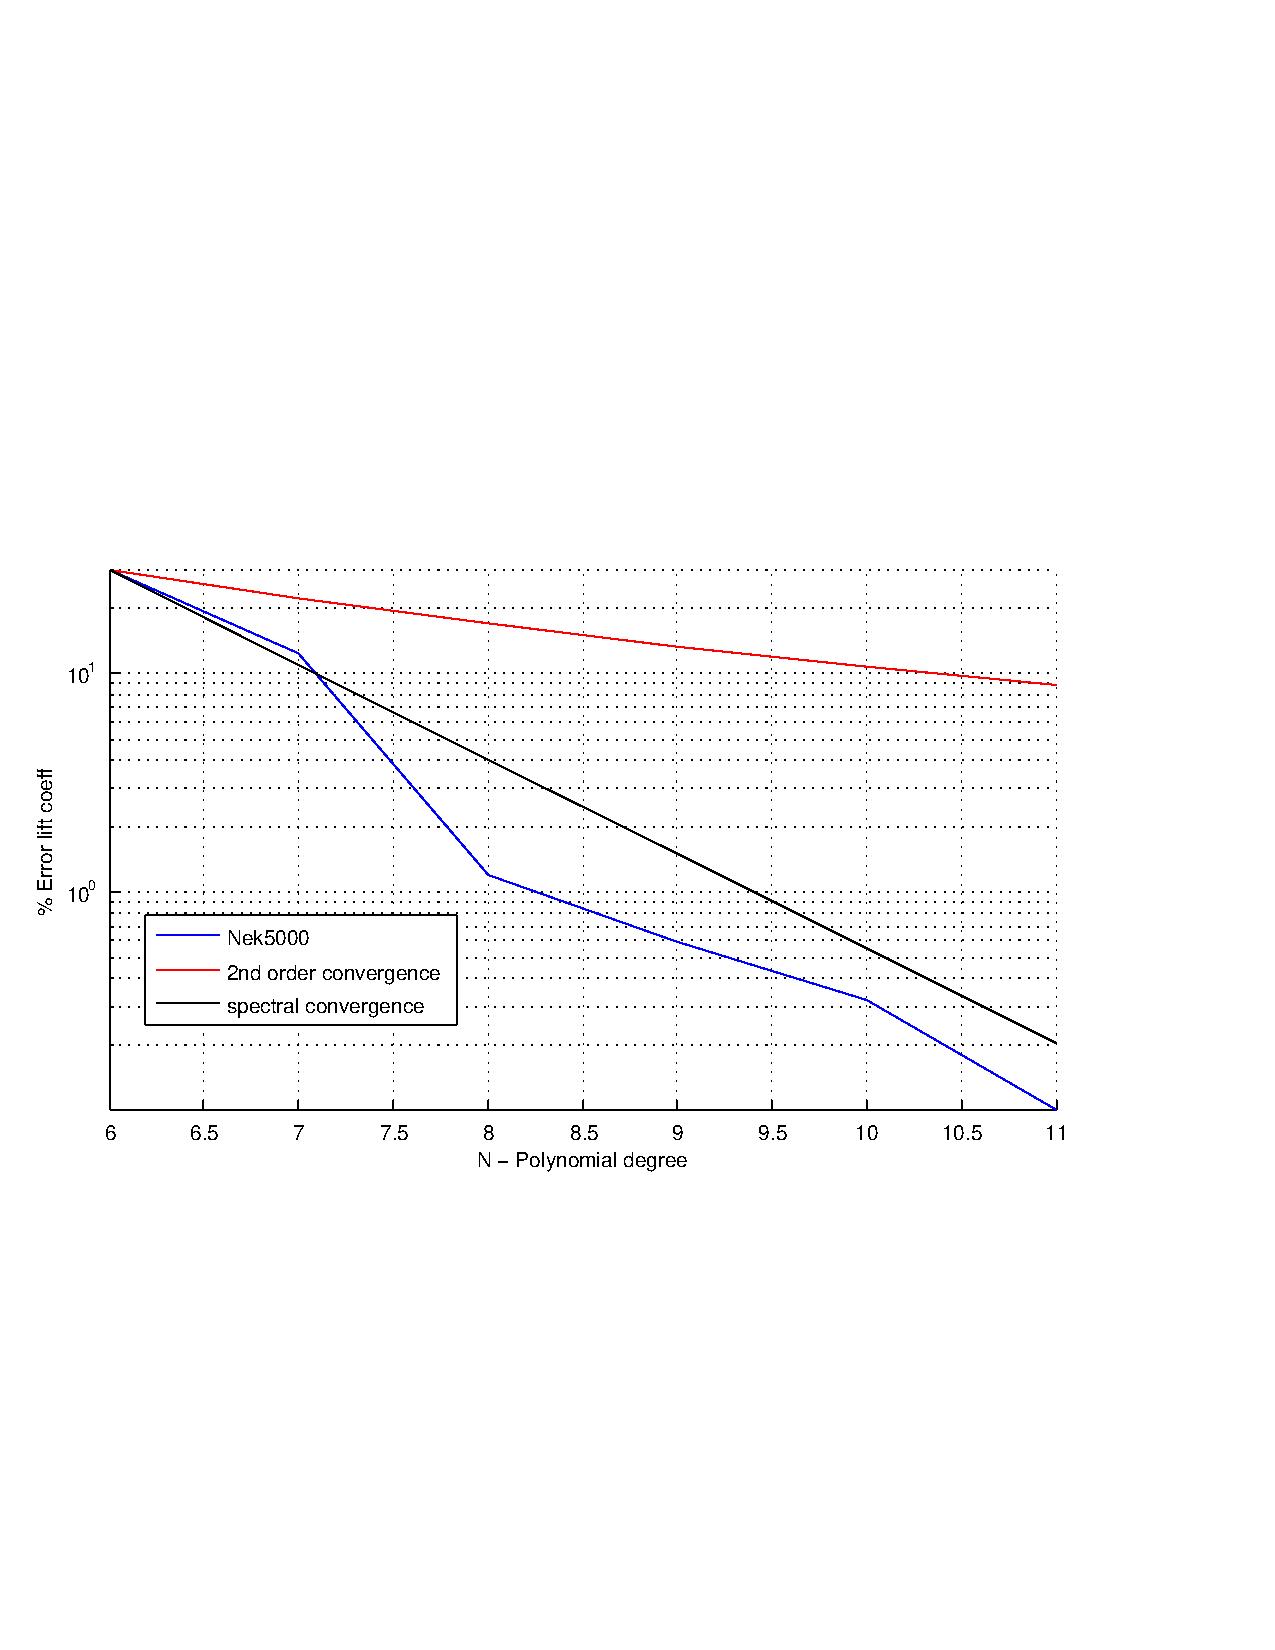
\includegraphics[trim=0.5cm 7cm 0.5cm 7cm, width=0.8\textwidth]{Figures/lift_coef4.pdf}}
	\caption{The logarithm of the error plotted against the polynomial degree. All results 
        are with $P_NP_{N-2}$ and dealiasing, and they are solved without using the 
    characteristic scheme or any filtering. A line illustrating a second order convergence is 
    plotted to illustrate the convergence rate.}
	\label{fig:liftconv}
\end{figure}
%

The setting that has the biggest impact on the result is the $P_NP_N$ scheme which clearly performs 
worse than the others. This is as expected since the discrete splitting is known to converge faster
for steady state flows. Notice however that by reducing the time-step the effect of the algebraic splitting
greatly reduces and achieves results of similar order as the discrete splitting.
Use of the IOFS method also has a negative effect on the accuracy,
this is also as expected because of the stability-accuracy trade-off for this method.
Remember that this scheme allows a much higher time step. The filtering is the least significant change
which confirms the analytical results from \eref{eq:filterenergy}. 
%
\begin{table}[h]
    \centering
    \begin{tabular}{c | c c c c c | c c }
         & \multicolumn{5}{|c|}{Settings} & \multicolumn{2}{|c}{\% Error} \\\hline
         \# & $\Delta t$ & ifsplit & Dealiasing & IOFS & Filter & $c_D$ & $c_L$ \\  \hline 
         1 & 6e-4& No & Yes& No & No & 0.005 & 0.10\\
         2 & 6e-4& No & Yes& No & Yes& 0.005 & 0.43\\
         3 & 6e-4& No & Yes& Yes& No & 0.005 & 0.18\\
         4 & 6e-4& No & No & No & No & 0.005 & 0.03\\
         5 & 6e-4& Yes& Yes& No & No & 0.012 & 2.35\\
         %6 & 4.5e-4& Yes& Yes& No & No & 0.015 & 0.01\\
         %7 & 3e-4& Yes& Yes& No & No & 0.018 & 0.01\\
    \end{tabular}
    %\begin{tabular}{c | c c c c | c c | c c c}
         %& \multicolumn{4}{|c|}{Settings} & \multicolumn{2}{|c|}{\% Error} & \multicolumn{3}{|c}{Data} \\\hline
         %\#  & ifsplit & Dealiasing & IOFS & Filter & $c_D$ & $c_L$ & DT & CFL & T/Tstep \\ \hline 
         %1 & F & T & F & F & 0.005 & 0.102 & 1e-04 & 2.03 & 2.1e-02 \\
         %2 & T & T & F & F & 0.013 & 2.349 & 1e-04 & 2.03 & 2.1e-02 \\
         %3 & F & T & F & T & 0.005 & 0.431 & 1e-04 & 2.03 & 2.1e-02 \\
         %4 & F & T & T & F & 0.005 & 0.179 & 1e-04 & 2.03 & 2.1e-02 \\
         %5 & F & F & F & F & NaN   & NaN   & 1e-04 & 2.03 & 2.1e-02 \\
    %\end{tabular}
    \caption{Test of solver settings in Nek5000.}
    \label{tab:perf}
\end{table}
%

Be aware that these results are obtained from a laminar test case and does not in any way 
suggest any optimal adjustment for Nek5000. An important example of this is the fact that 
deactivating de-aliasing yields better results. For a coarser mesh or a more turbulent flow 
this would not be the case, and that the result is better is probably due to 
the accuracy, which are close to the accuracy given by the reference solution. 
The resuslts do however give an indication to the general effect of these settings that 
are worth noticing.

%----------------------------------------------------------------------------------------
\chapter{Concluding remarks}
Nek5000 has proven to give accurate results with a relatively coarse mesh as
presented in~\cref{results}. This is as expected since it is based on a higher order 
method known to yield great accuracy. As for the performance it is no doubt that the 
efforts put into the efficiency of the code has paid off. The possibility to obtain 
results 5-10 times faster than similar softwares is an important factor to keep in mind. 
The polynomial degree is chosen by changing a single parameter, which makes performance tests
and accuracy adjustments simple to do. 

Since the mathematical formulation in Nek5000 is based on a tensor product of the basis functions 
in each direction it is limited to the use of hex-mesh. This is no problem for the geometries 
studied in this thesis, but for complex geometry the use of tetrahedral mesh is mandatory.
It did also prove difficult to work with refinements made in ICEM which restricts the possibility 
to make a mesh with large differences in grid size.

Another aspect worth noticing is the filtering procedure which has some similarities to variational multiscale
as presented in~\cref{physfilt}. It would be interesting to design some test cases to further 
investigate its properties. 

The fact that Nek5000 is an open-source code is also a huge advantage to other black-box solvers. 
Although the user community is not that large there are several commited users that provide 
their help on short notice. Many different examples are available, and the user guide 
contains a nice introduction with everything needed to get the program up and running. 
The documentation of variables and functions are sometimes missing, which is the main motivation 
to create Appendix~\ref{AppendixB}. 


\section{Further work}
The surface projection could be expanded and improved in many ways. Making it iterative 
to make sure the GLL-points are distributed correspondingly, The norm corresponding
to the normal is prone to give errors and should be calculated based on points further away\ldots.
For the simple array case it was experimented with different meshes and the refinement procedure 
in ICEM quickly leads to small elements with wide angles which tends to lead to problems 
in Nek5000. The author do however believe that by making an ogrid around the most important part of 
the domain, say for instance the box, $x/H < 3,\: |y|/H < 0.4,\: z/H < 0.15$ the nodes could have been 
distributed in a more economical fashion and an overall better result could have been achieved.


\colorbox{green}{How did Nek5000 perform overall, user-friendly ?,correctness,speed etc.}

 
%\input{Chapters/Chapter5} 
%\input{Chapters/Chapter6} 
%\input{Chapters/Chapter7} 

%----------------------------------------------------------------------------------------
%	THESIS CONTENT - APPENDICES
%----------------------------------------------------------------------------------------

%\addtocontents{toc}{\vspace{2em}} % Add a gap in the Contents, for aesthetics

%\appendix % Cue to tell LaTeX that the following 'chapters' are Appendices

%% Include the appendices of the thesis as separate files from the Appendices folder
%% Uncomment the lines as you write the Appendices

%% Appendix A

\chapter{Fundamental basics of numerical analysis} % Main appendix title

\label{AppendixA} % For referencing this appendix elsewhere, use \ref{AppendixA}

\lhead{Appendix A. \emph{Numerical analysis}} % This is for the header on each page - perhaps a shortened title

\section{GLL-quadrature}
\section{Essential polynomials}
\begin{enumerate}
    \item Legendre polynomials
    \item Lagrange basis 
\end{enumerate}

\section{Preliminary concepts}

\begin{enumerate}
    \item coersiveness
    \item Bounded  
\end{enumerate}

\section{Lax-Milgram theorem}

Stating the theroem without proof 


%%% Appendix Template

\chapter{Variables and Functions in Nek5000} % Main appendix title

\label{AppendixB} % Change X to a consecutive letter; for referencing this appendix elsewhere, use \ref{AppendixX}

\lhead{Appendix B. \emph{Variables and functions in Nek}} % Change X to a consecutive letter; this is for the header on each page - perhaps a shortened title

\section{Variables}

\section{Functions}

%%\input{Appendices/AppendixC}

%\addtocontents{toc}{\vspace{2em}} % Add a gap in the Contents, for aesthetics

%\backmatter

%----------------------------------------------------------------------------------------
%	BIBLIOGRAPHY
%----------------------------------------------------------------------------------------

\label{Bibliography}

\lhead{\emph{Bibliography}} % Change the page header to say "Bibliography"

\bibliographystyle{unsrtnat} % Use the "unsrtnat" BibTeX style for formatting the Bibliography

\bibliography{Bibliography} % The references (bibliography) information are stored in the file named "Bibliography.bib"

\end{document}  
